\chapter{Appendix}
\label{chap:appendix}

This appendix provides supplementary materials that support the methodological transparency, reproducibility, and interpretability of the profile-aware dark pattern auditing framework. While the main body of the report focuses on the conceptual framework, experimental design, major findings, and statistical interpretation, the appendix collects the complete profile settings, keyword pools, annotation guidelines, full visualization outputs, convergence evidence, and statistical validation tables. These materials are intended to make the auditing procedure more transparent and to allow readers to understand how profile-conditioned exposure was operationalized and evaluated.

\begin{figure}[htbp]
    \centering
    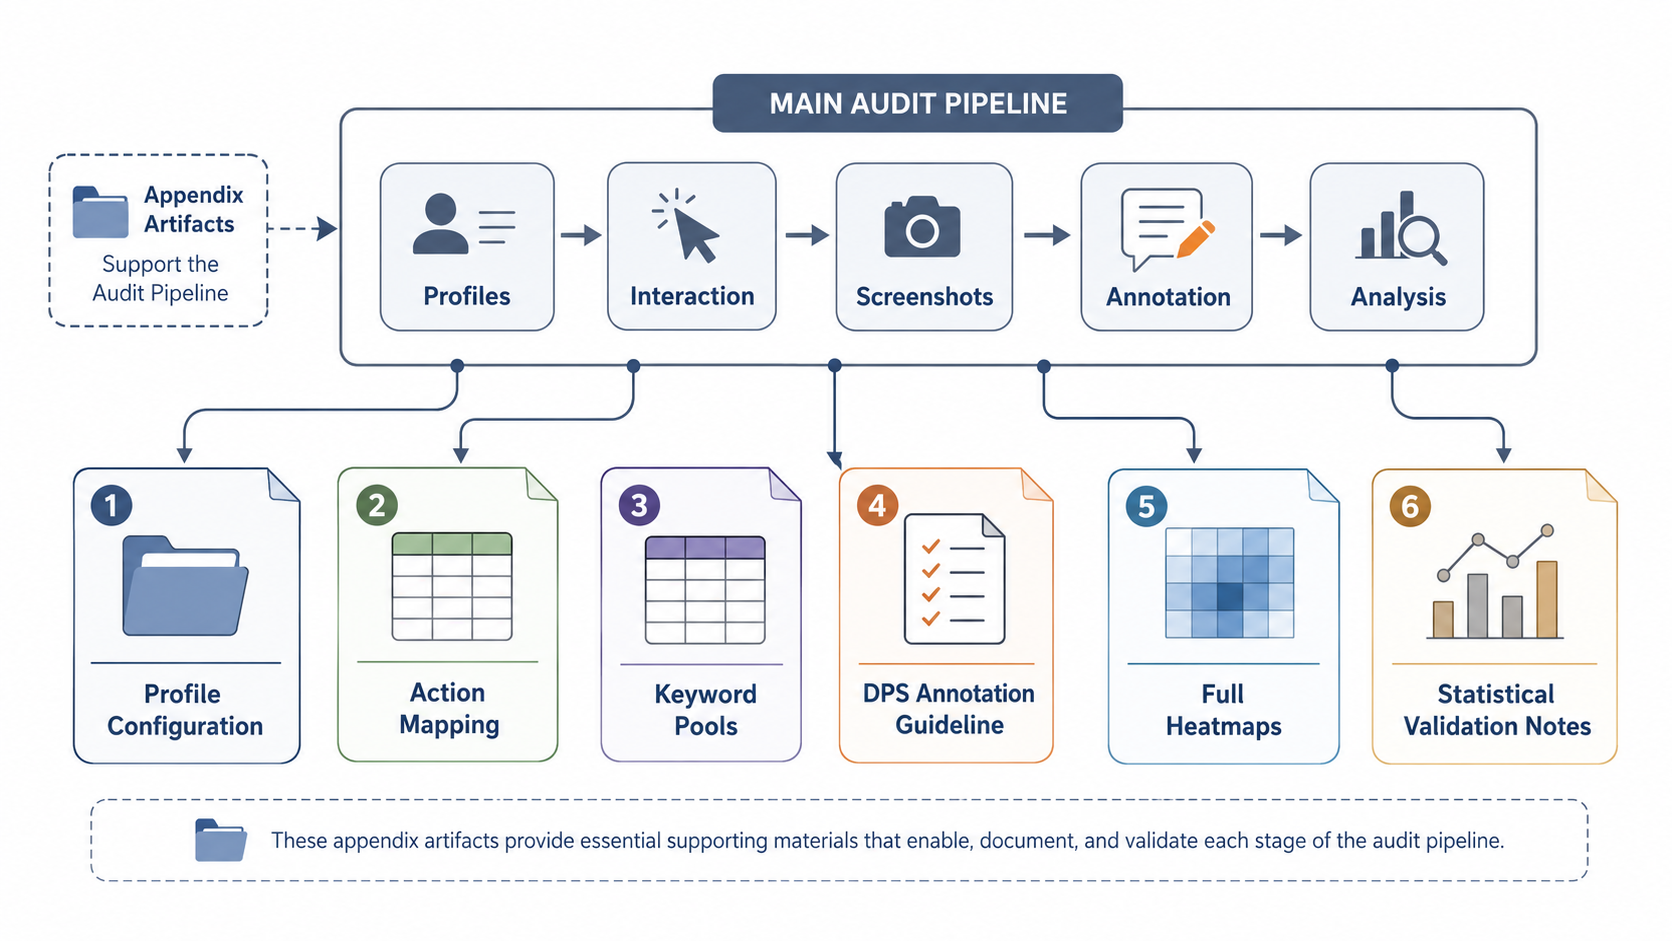
\includegraphics[width=0.95\linewidth]{figures/pictures/appendix_artifact_index.png}
    \caption{Appendix Artifact Index}
    \label{fig:appendix-artifact-index}
\end{figure}

\section{Appendix A: Full Profile Configuration}
\label{app:profile-configuration}

Appendix A reports the full controlled profile configuration used in the audit experiment. Each profile is represented by a behavior distribution over a fixed set of interaction actions. These probabilities are not intended to model any real demographic group. Instead, they define reproducible experimental agents with different interaction tendencies. In this project, the profiles are constructed from controllable interests and behaviors, while demographic attributes are deliberately excluded to reduce ethical and reproducibility concerns.

Table~\ref{tab:profile-behavior-probabilities-appendix} summarizes the behavior probabilities for the three controlled profiles: the high-payment shopping profile, the low-payment browsing profile, and the bargain-hunter profile. The probabilities sum to one within each profile.

The table reports the conceptual action space after collapsing the operational actions used in implementation back into the four high-level categories defined in Chapter~\ref{sec:conceptual-framework}. The mapping from implementation-level actions to conceptual categories is listed in Table~\ref{tab:action-mapping}.

\begin{table}[htbp]
    \centering
    \caption{Behavior probability configuration for controlled user profiles.}
    \label{tab:profile-behavior-probabilities-appendix}
    \begin{tabular}{lccc}
        \toprule
        \textbf{Interaction Action} & 
        \textbf{High-Payment Shopping} & 
        \textbf{Low-Payment Browsing} & 
        \textbf{Bargain Hunter} \\
        \midrule
        Visit homepage & 0.05 & 0.15 & 0.10 \\
        Search keyword & 0.25 & 0.15 & 0.35 \\
        Browse or scroll page & 0.40 & 0.60 & 0.35 \\
        Decision-interface visit & 0.30 & 0.10 & 0.20 \\
        \midrule
        Total & 1.00 & 1.00 & 1.00 \\
        \bottomrule
    \end{tabular}
\end{table}

The high-payment shopping profile is designed to represent an interaction pattern with stronger purchase intent. It searches for high-value products, browses product pages, and more frequently enters decision interfaces such as payment pages, membership pages, or checkout-related screens. The low-payment browsing profile is designed to represent a lower-intent browsing pattern, with more time spent on homepage exploration and general scrolling, and fewer visits to payment-related interfaces. The bargain-hunter profile represents a promotion-sensitive pattern, with stronger attention to discounts, coupons, flash sales, group-buying, and reward mechanisms.

\section{Appendix A.1: Action Mapping}
\label{app:action-mapping}

Table~\ref{tab:action-mapping} maps the implementation-level action set to the four conceptual categories used in the main framework. This mapping is used for analysis and reporting so that fine-grained operational traces can be compared within a shared abstraction.

\begin{table}[htbp]
    \centering
    \caption{Mapping from fine-grained actions to conceptual action categories.}
    \label{tab:action-mapping}
    \small
    \setlength{\tabcolsep}{4pt}
    \renewcommand{\arraystretch}{1.08}
    \begin{tabularx}{\textwidth}{@{}p{3.4cm}p{2.3cm}X@{}}
        \toprule
        \textbf{Fine-grained action} & \textbf{High-level category} & \textbf{Explanation} \\
        \midrule
        \texttt{visit\_homepage} & home & Visits the homepage or returns to the main interface. \\
        \texttt{search\_keyword} & search & Enters a keyword and triggers keyword-based search. \\
        \texttt{browse\_or\_scroll\_page} & browse & Scrolls through or passively explores ordinary content. \\
        \texttt{click\_recommended\_item} & browse & Opens a recommended item during exploratory browsing. \\
        \texttt{like\_or\_favorite} & browse & Expresses lightweight engagement while staying in content exploration. \\
        \texttt{follow\_account} & browse & Follows an account or creator without entering a decision flow. \\
        \texttt{stay\_on\_content} & browse & Remains on content and continues passive exposure to the current feed or page. \\
        \texttt{decision\_interface\_visit} & decision & Enters checkout, subscription, membership, payment, or confirmation interfaces. \\
        \texttt{close\_popup} & home & Dismisses an interruption and returns to the underlying page or main interface. \\
        \texttt{back} & home & Navigates back to the previous page or a higher-level interface. \\
        \bottomrule
    \end{tabularx}
\end{table}

\section{Appendix B: Keyword Pools}
\label{app:keyword-pools}

Appendix B provides the keyword pools used to instantiate the interest component of each controlled profile. In the proposed framework, user interests are modeled as probability distributions over keyword categories. During the interaction process, when the sampled action is the fine-grained \texttt{search\_keyword} action, the system selects a keyword from the corresponding profile-specific keyword pool. This design makes the profile construction controllable and reproducible while still allowing different profiles to generate different interaction traces.

In the operational implementation, this search step corresponds to the fine-grained \texttt{search\_keyword} action, which is mapped back to the conceptual \(\mathrm{search}\) category before analysis.

Table~\ref{tab:keyword-pools} summarizes the keyword categories used by the three profiles.

\begin{table}[htbp]
    \centering
    \caption{Keyword pools for controlled profile construction.}
    \label{tab:keyword-pools}
    \begin{tabular}{lp{9cm}}
        \toprule
        \textbf{Profile} & \textbf{Keyword Categories} \\
        \midrule
        High-payment shopping & 
        High-value goods; premium electronics; luxury skincare; membership services. \\
        \addlinespace
        Low-payment browsing & 
        Daily necessities; casual browsing; snacks; home supplies. \\
        \addlinespace
        Bargain hunter & 
        Discount; coupon; flash sale; group-buy; membership rewards. \\
        \bottomrule
    \end{tabular}
\end{table}

The keyword pools are not intended to exhaustively represent all possible user interests. Rather, they serve as controlled stimuli for auditing whether different interest-behavior configurations are associated with different dark pattern exposure patterns. The implementation files provide the exact keywords used for each category, the sampling probabilities assigned to each keyword group, and examples of generated search instructions.

\section{Appendix C: DPS Annotation Guideline}
\label{app:dps-annotation-guideline}

Appendix C documents the annotation guideline for the seven-dimensional Dark Pattern Score vector, denoted as
\[
DPS = [I, F, P, C, S, N, FA],
\]
where \(I\) refers to Interface Interference, \(F\) to Friction, \(P\) to Pressure, \(C\) to Contextual Deception, \(S\) to Sneaking, \(N\) to Nagging, and \(FA\) to Forced Action. The purpose of this guideline is to improve annotation consistency and make clear how each dimension should be interpreted during screenshot-level labeling.

Table~\ref{tab:dps-guideline} provides the annotation guideline used to interpret the seven DPS dimensions. Detailed examples from collected screenshots are reported in the main DPS chapter where appropriate.

\begin{table}[htbp]
    \centering
    \caption{DPS annotation guideline for mixed numeric exposure scores.}
    \label{tab:dps-guideline}
    \footnotesize
    \setlength{\tabcolsep}{3pt}
    \renewcommand{\arraystretch}{1.06}
    \begin{tabularx}{\textwidth}{@{}p{1.75cm}XXXX@{}}
        \toprule
        \textbf{DPS Dimension} &
        \textbf{Definition} &
        \textbf{Positive Examples} &
        \textbf{Negative Examples} &
        \textbf{Boundary Cases} \\
        \midrule
        Interface Interference \((I)\) &
        Visual or structural design that steers user attention or makes one option more salient than alternatives. &
        A large highlighted ``Buy Now'' button; a visually hidden decline option; misleading button hierarchy. &
        A neutral interface where accept and reject options are equally visible. &
        A visually attractive button is not labeled as interference unless it meaningfully distorts choice visibility or salience. \\
        \addlinespace

        Friction \((F)\) &
        Additional steps, effort, or difficulty imposed on the user when attempting to decline, cancel, close, or avoid an action. &
        Multiple screens required to cancel; difficult unsubscribe path; repeated confirmation before refusal. &
        A single clear cancel or close button. &
        Extra steps may be functional rather than deceptive if they are necessary for security or irreversible actions. \\
        \addlinespace

        Pressure \((P)\) &
        Interface language or timing mechanisms that create urgency, scarcity, social pressure, or emotional pressure. &
        Countdown timers; ``only 2 left'' messages; ``many users are buying now'' prompts; emotionally loaded warnings. &
        Plain factual product information without urgency or emotional manipulation. &
        A real time-limited promotion should be annotated carefully if the interface exaggerates urgency or obscures conditions. \\
        \addlinespace

        Contextual Deception \((C)\) &
        A mismatch between the apparent meaning of an interface element and the actual consequence of interacting with it. &
        A close button that opens another promotion; a misleading checkbox; a button label that hides subscription consequences. &
        A clearly labeled button whose result matches user expectation. &
        Ambiguous icons should be annotated only when the surrounding context suggests a misleading or deceptive interpretation. \\
        \addlinespace

        Sneaking \((S)\) &
        Hidden or delayed disclosure of costs, conditions, subscriptions, add-ons, or data-related consequences. &
        Hidden fees added near checkout; preselected add-ons; unclear membership renewal terms. &
        Fully disclosed price, fee, and subscription information before user commitment. &
        Additional charges are not labeled as sneaking if they are clearly disclosed before the decision point. \\
        \addlinespace

        Nagging \((N)\) &
        Repeated interruptions or prompts that ask the user to perform an action unrelated to the immediate task. &
        Repeated pop-ups for membership, notification permission, app rating, or promotion after dismissal. &
        A single relevant reminder that does not interrupt the task flow. &
        Repetition should be considered in relation to interaction history; a single prompt may become nagging if it repeatedly reappears after refusal. \\
        \addlinespace

        Forced Action \((FA)\) &
        A design that requires the user to perform an additional action, registration, permission grant, or commitment before continuing. &
        Mandatory login before browsing; forced app permission; required membership prompt before accessing core content. &
        Optional login or permission request that can be skipped without blocking the task. &
        Some forced actions may be functionally necessary, such as payment authentication; these should be distinguished from unnecessary coercive barriers. \\
        \bottomrule
    \end{tabularx}
\end{table}

The scoring scheme combines binary indicators and numeric exposure scores. Pressure, Contextual Deception, Sneaking, and Forced Action are typically treated as binary labels in the present dataset. Interface Interference, Friction, and Nagging may use ordinal levels or counts when the annotation protocol distinguishes weak from strong exposure, additional effort, or repeated interruption. Occurrence-rate analysis uses \(D_i>0\), while intensity analysis uses raw score means.

\section{Appendix D: Full Heatmaps}
\label{app:full-heatmaps}

Appendix D provides the complete set of DPS heatmaps for all audited applications and profiles. In the main report, only representative heatmaps are shown to illustrate the most important exposure patterns. The appendix includes the full visualization set so that readers can inspect the distribution of dark pattern exposure across the complete experimental scope.

Each heatmap uses the DPS dimensions as one axis and either applications, profiles, or application categories as the other axis, depending on the visualization design. These heatmaps are intended to support the main finding that different profiles show different exposure patterns. They also allow readers to identify which DPS dimensions are more prominent in particular app categories.

\begin{figure}[htbp]
    \centering
    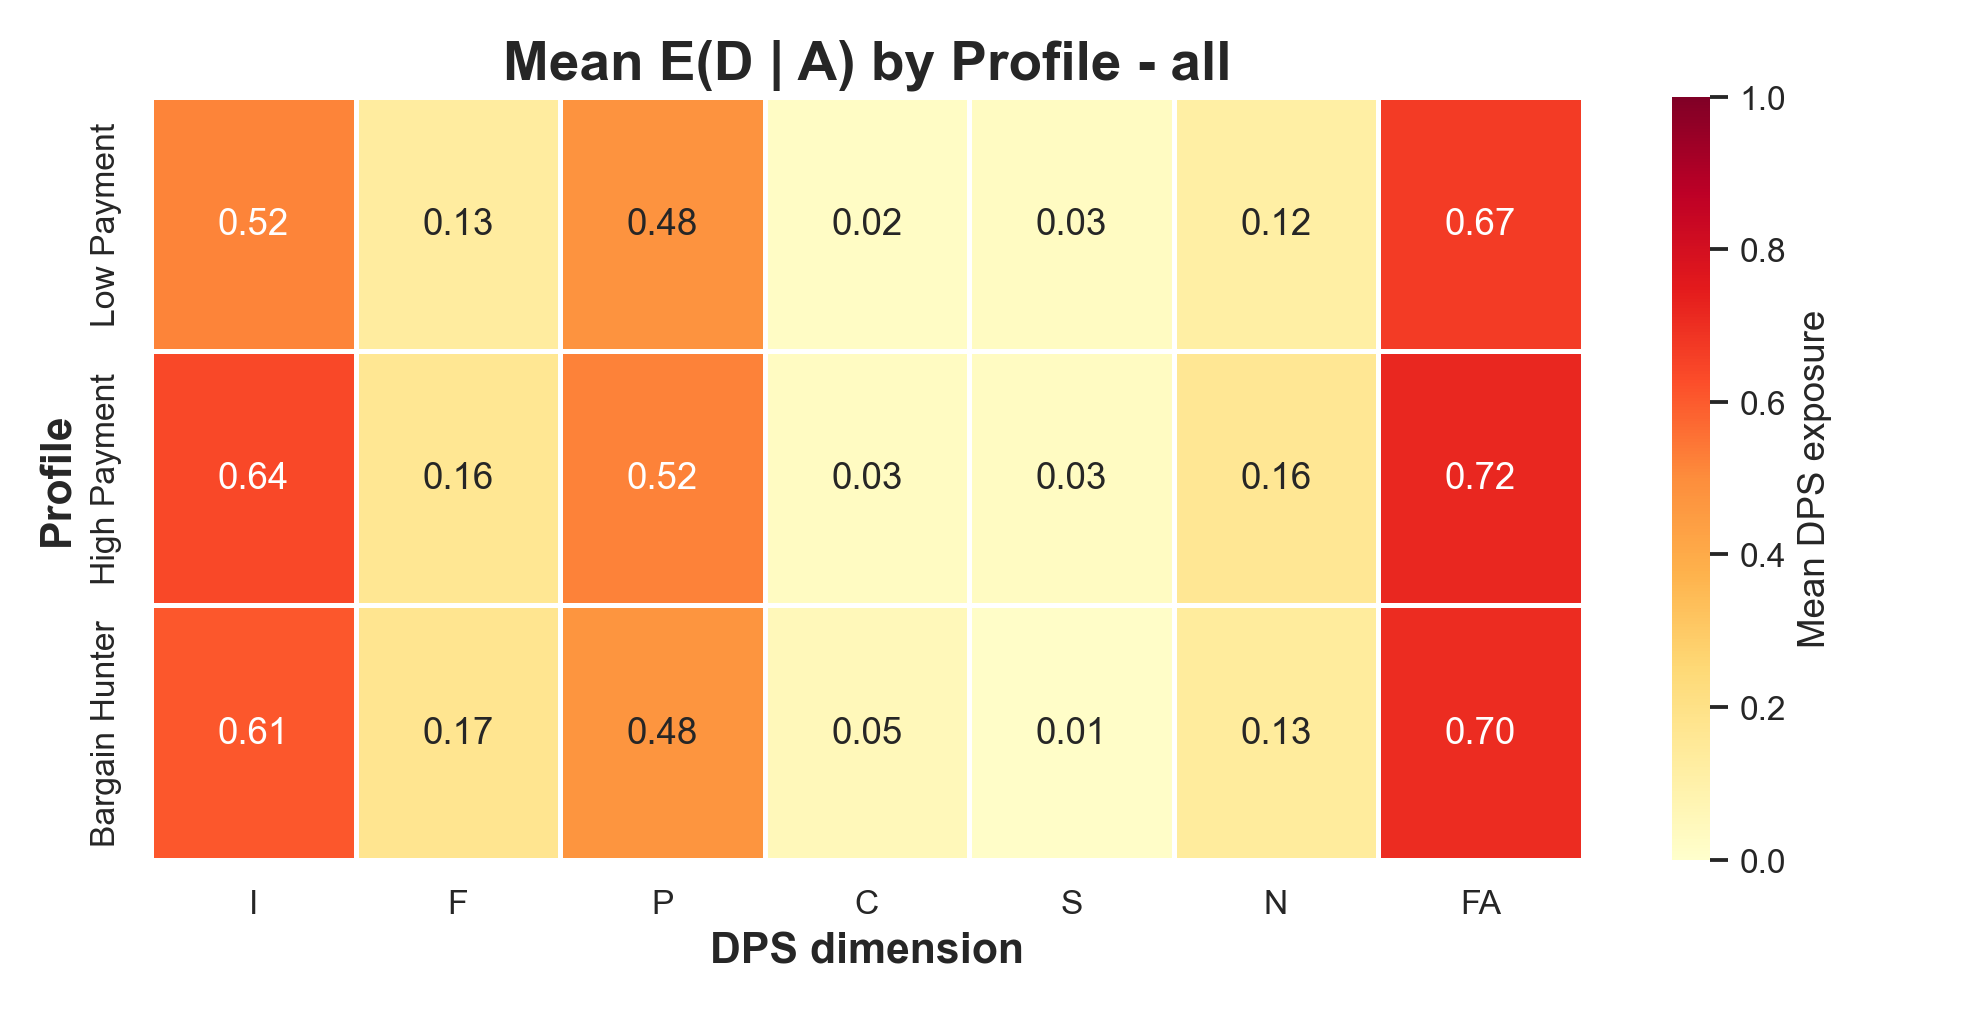
\includegraphics[width=0.95\linewidth]{figures/statistics/heatmap_mean_exposure_all.png}
    \caption{Complete raw DPS intensity mean heatmap for all applications and controlled profiles.}
    \label{fig:full-heatmap-all}
\end{figure}

\begin{figure}[htbp]
    \centering
    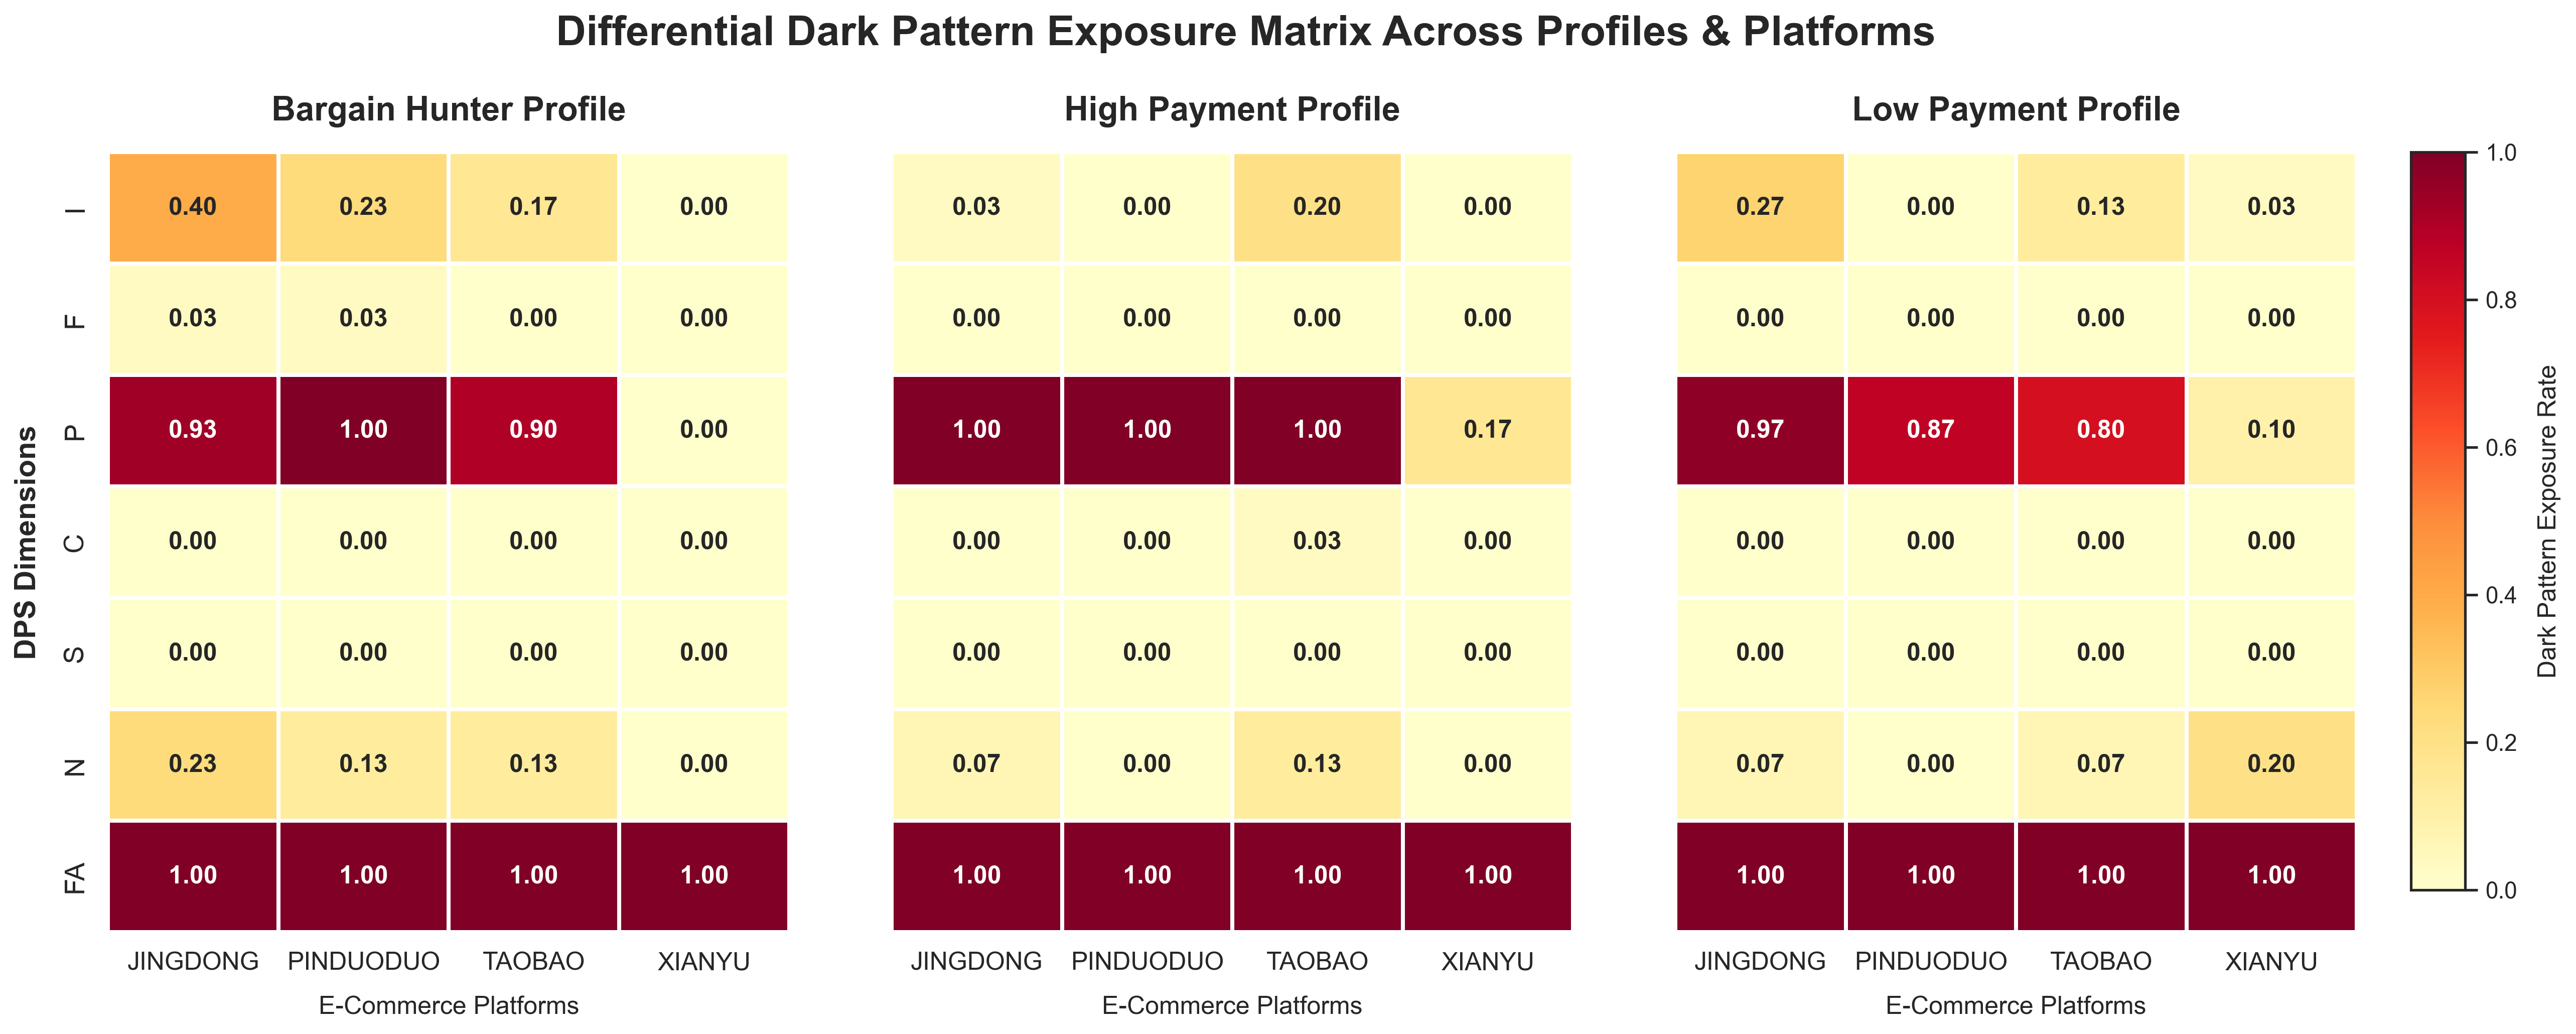
\includegraphics[width=0.95\linewidth]{figures/heatmap_shopping.png}
    \caption{Detailed raw DPS intensity heatmap for shopping applications.}
    \label{fig:heatmap-shopping-detail}
\end{figure}

\begin{figure}[htbp]
    \centering
    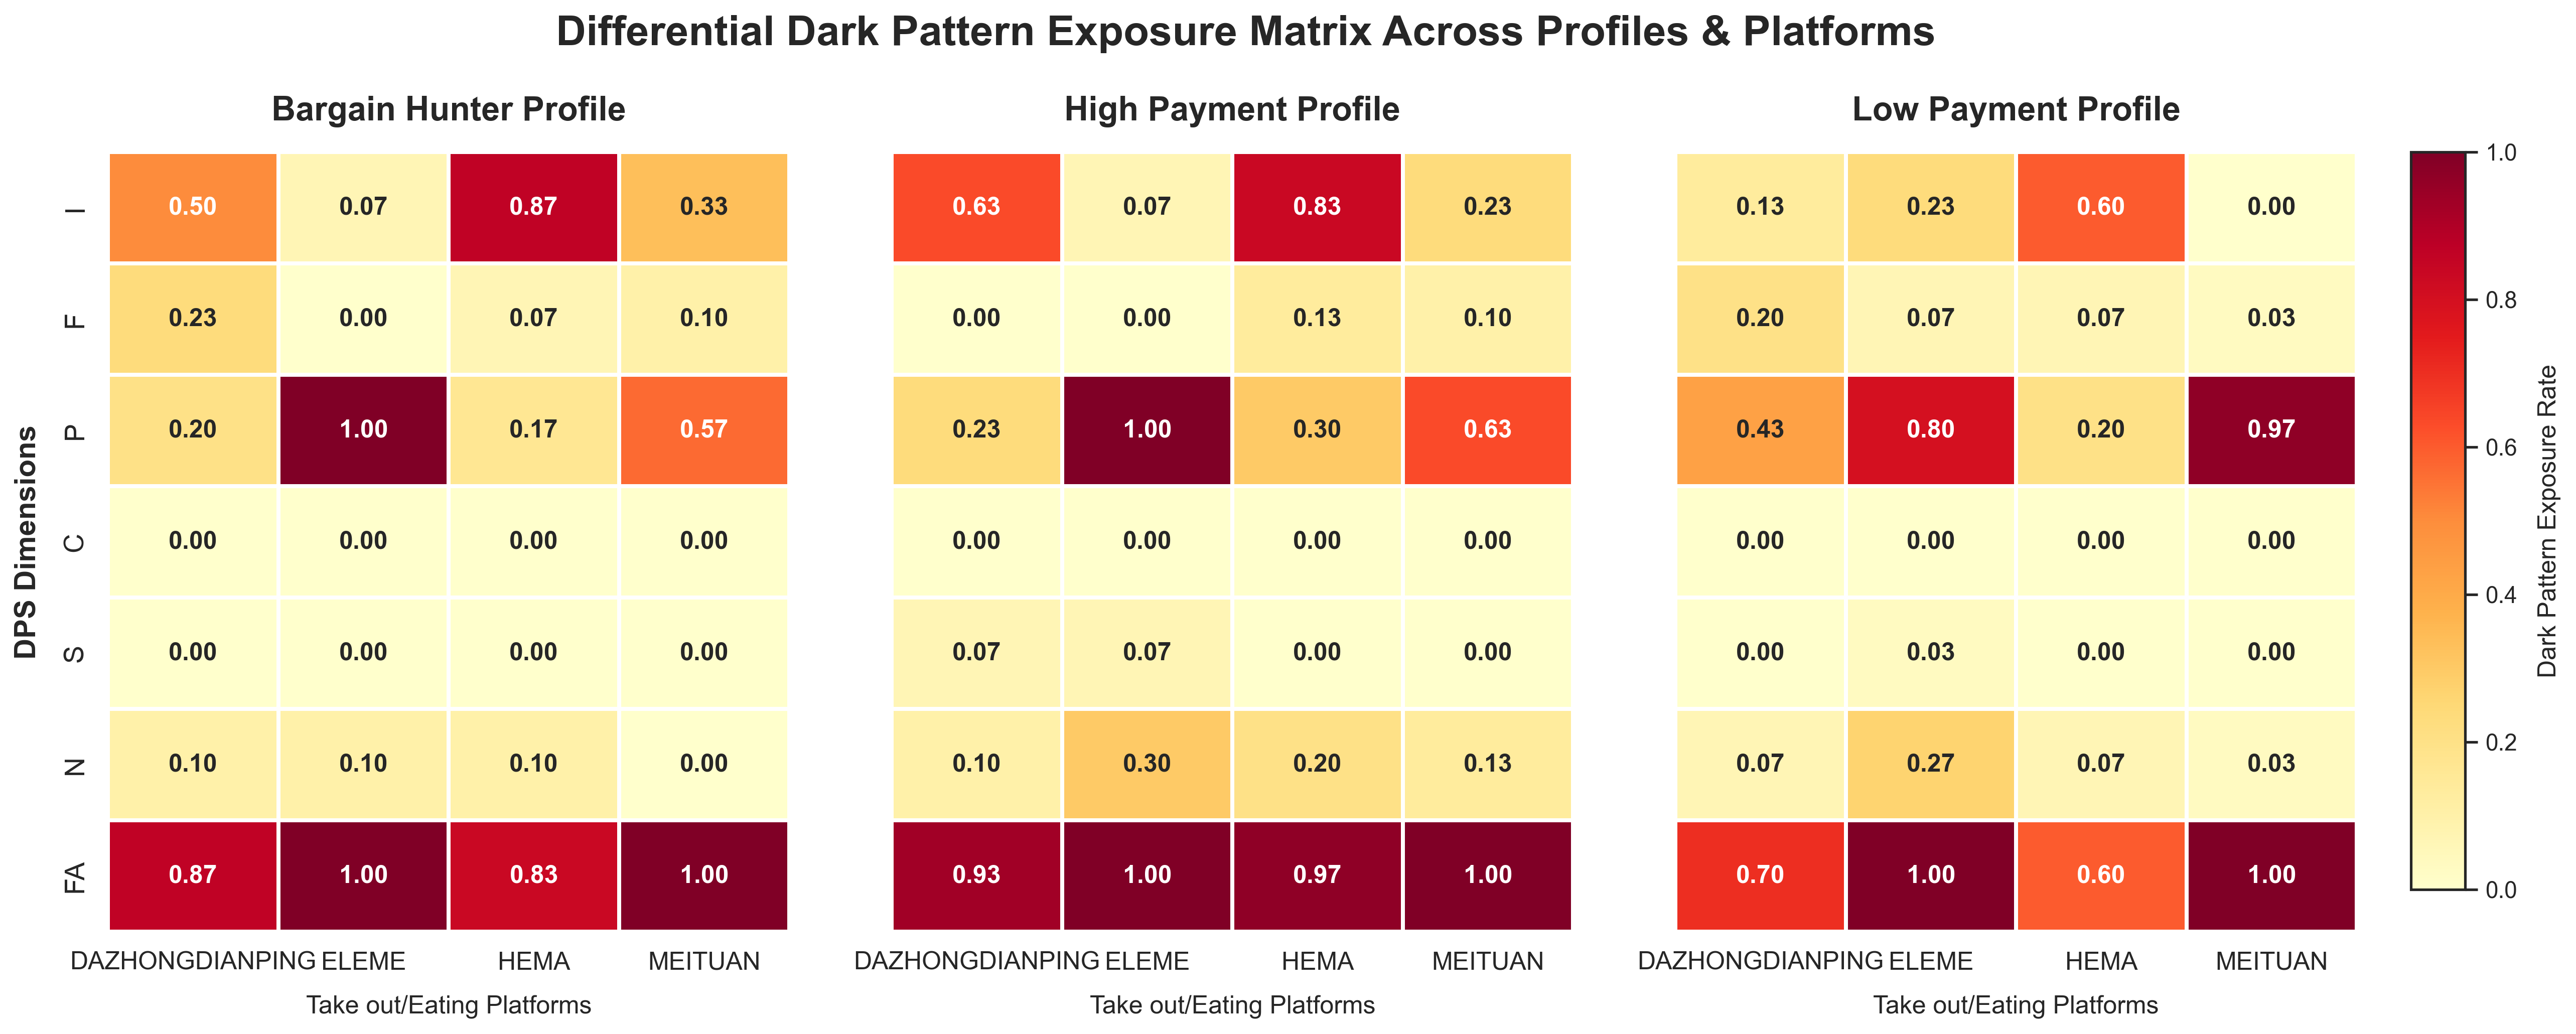
\includegraphics[width=0.95\linewidth]{figures/heatmap_eating.png}
    \caption{Detailed raw DPS intensity heatmap for food-delivery and eating-related applications.}
    \label{fig:heatmap-eating-detail}
\end{figure}

\begin{figure}[htbp]
    \centering
    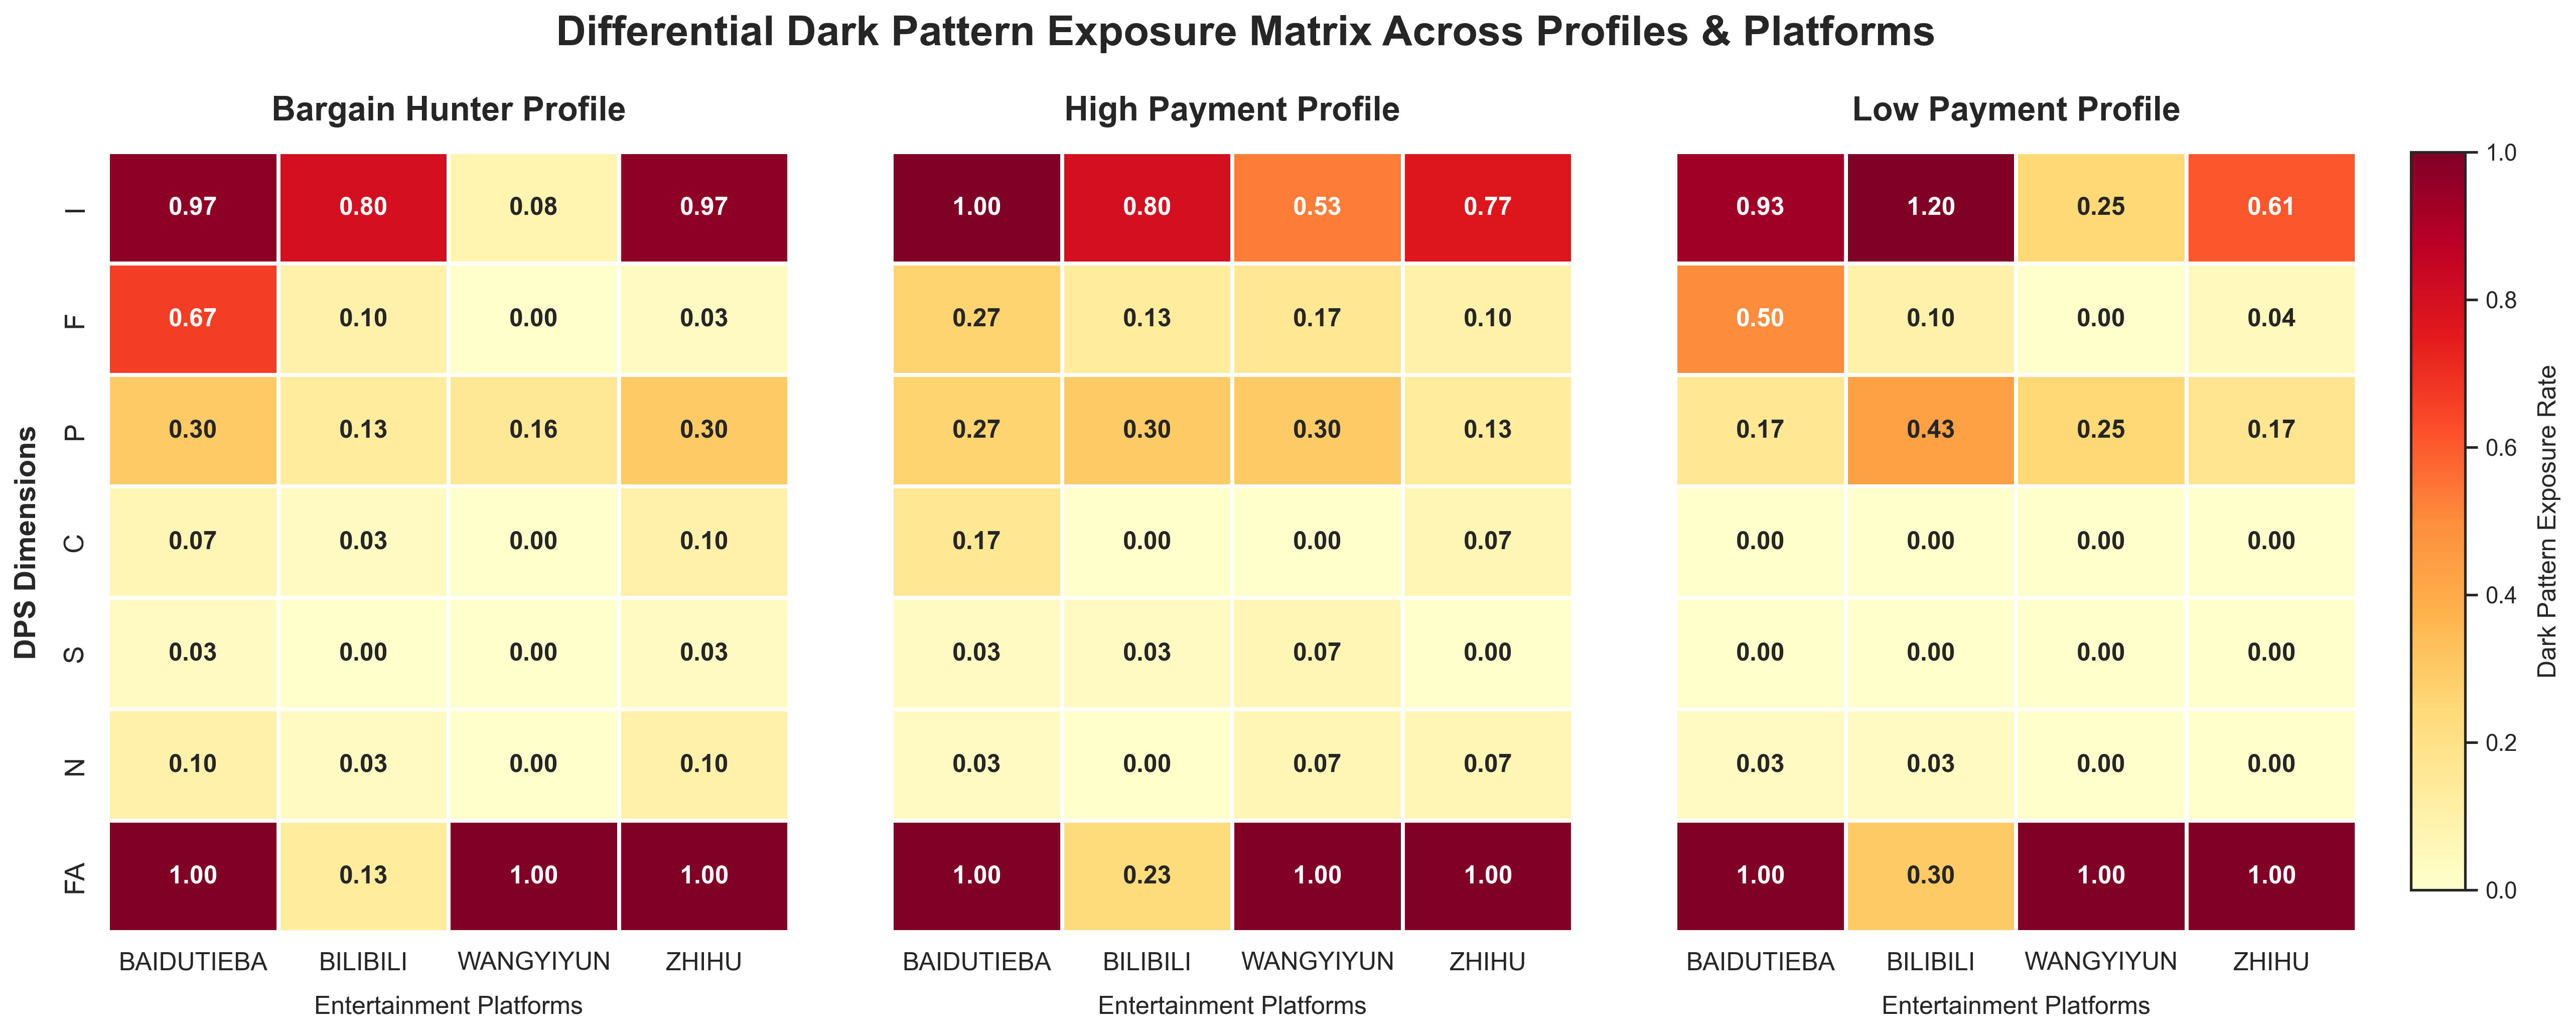
\includegraphics[width=0.95\linewidth]{figures/heatmap_entertainment.png}
    \caption{Detailed raw DPS intensity heatmap for entertainment applications.}
    \label{fig:heatmap-entertainment-detail}
\end{figure}

\begin{figure}[htbp]
    \centering
    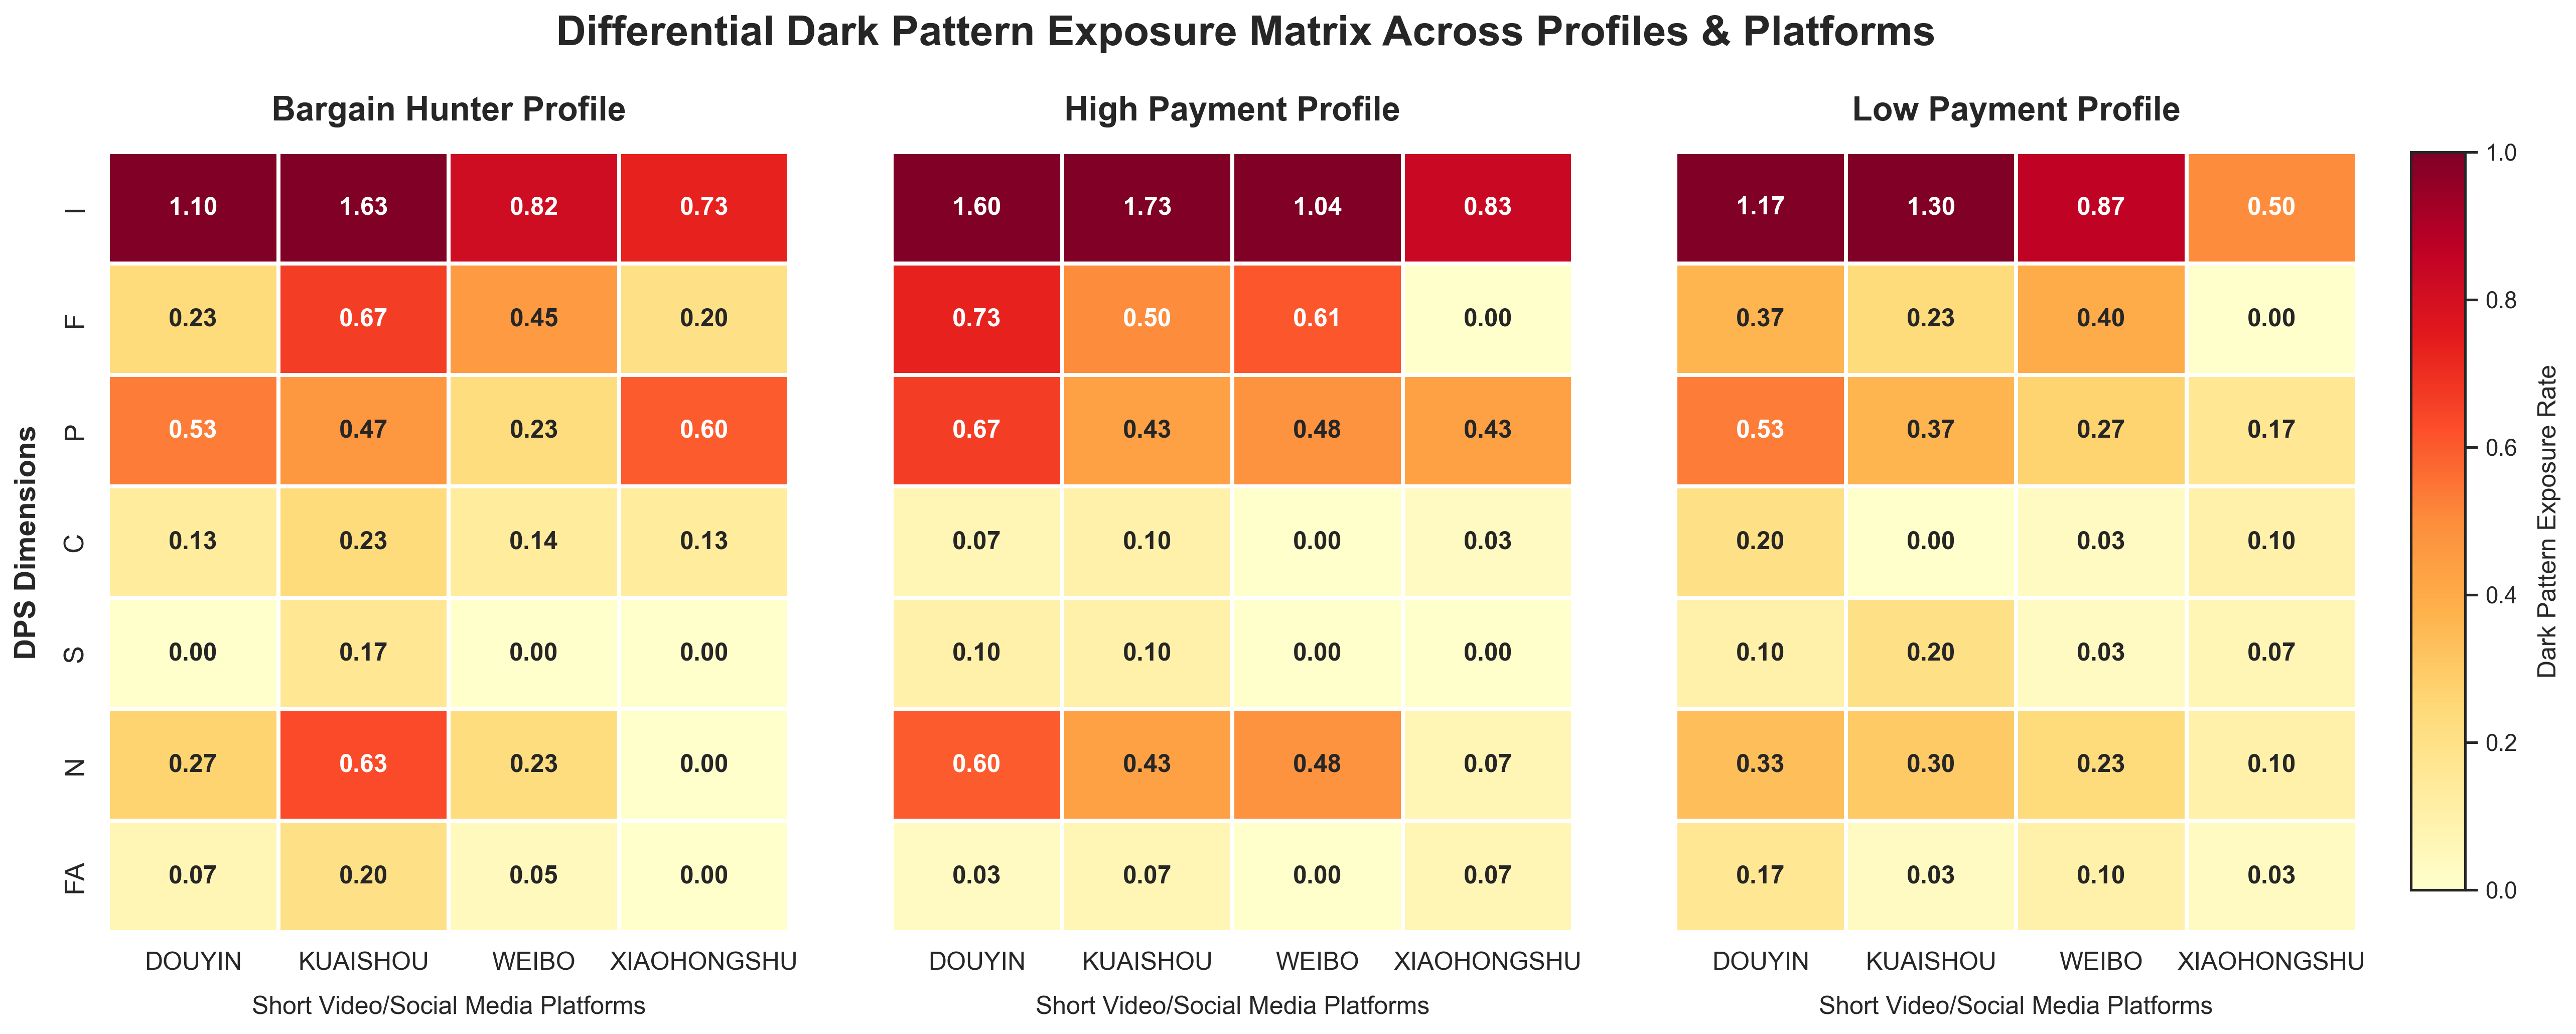
\includegraphics[width=0.95\linewidth]{figures/heatmap_social.png}
    \caption{Detailed raw DPS intensity heatmap for social applications.}
    \label{fig:heatmap-social-detail}
\end{figure}

The captions in this appendix describe what each heatmap represents without restating unsupported causal claims. The text uses careful language such as ``the heatmap indicates higher observed exposure'' or ``the pattern suggests profile-associated differences in exposure.''

\section{Appendix E: Statistical Visualization Set}
\label{app:statistical-visualizations}

Appendix E includes the complete statistical visualization set currently exported by the analysis pipeline. These figures complement the main report by showing q-value patterns, permutation-test summaries, observed L1 distances, Cramér's \(V\) association strengths, and running mean convergence curves.

For a DPS dimension \(d\), the running mean after \(t\) interaction steps can be written as
\[
\bar{D}_{A,d}^{(t)} = \frac{1}{t}\sum_{\tau=1}^{t} D_{A,d}^{(\tau)},
\]
where \(A\) denotes the controlled profile and \(D_{A,d}^{(\tau)}\) denotes the observed DPS label for dimension \(d\) at step \(\tau\).

\subsection{Running Mean Convergence Curves}
\label{app:running-mean-curves}

The following running mean convergence curves collect the full set of exported line plots from the analysis pipeline. They are grouped by application category and arranged in four columns so that several curves appear on each row.

\newcommand{\curvecell}[1]{%
    \begin{minipage}[t]{0.24\textwidth}
        \centering
        \includegraphics[width=\linewidth]{#1}
    \end{minipage}%
}

\subsubsection{Shopping}
\noindent
\curvecell{figures/statistics/curves_shopping/curve_E_bargain_hunter_jingdong_shopping.png}\hfill
\curvecell{figures/statistics/curves_shopping/curve_E_bargain_hunter_pinduoduo_shopping.png}\hfill
\curvecell{figures/statistics/curves_shopping/curve_E_bargain_hunter_taobao_shopping.png}\hfill
\curvecell{figures/statistics/curves_shopping/curve_E_bargain_hunter_xianyu_shopping.png}

\par\medskip

\noindent
\curvecell{figures/statistics/curves_shopping/curve_E_high_payment_shopping_jingdong_shopping.png}\hfill
\curvecell{figures/statistics/curves_shopping/curve_E_high_payment_shopping_pinduoduo_shopping.png}\hfill
\curvecell{figures/statistics/curves_shopping/curve_E_high_payment_shopping_taobao_shopping.png}\hfill
\curvecell{figures/statistics/curves_shopping/curve_E_high_payment_shopping_xianyu_shopping.png}

\par\medskip

\noindent
\curvecell{figures/statistics/curves_shopping/curve_E_low_payment_browsing_jingdong_shopping.png}\hfill
\curvecell{figures/statistics/curves_shopping/curve_E_low_payment_browsing_pinduoduo_shopping.png}\hfill
\curvecell{figures/statistics/curves_shopping/curve_E_low_payment_browsing_taobao_shopping.png}\hfill
\curvecell{figures/statistics/curves_shopping/curve_E_low_payment_browsing_xianyu_shopping.png}

\par\medskip

\subsubsection{Eating}
\noindent
\curvecell{figures/statistics/curves_eating/curve_E_bargain_hunter_DaZhongDianPing_eating.png}\hfill
\curvecell{figures/statistics/curves_eating/curve_E_bargain_hunter_ELeMe_eating.png}\hfill
\curvecell{figures/statistics/curves_eating/curve_E_bargain_hunter_HeMa_eating.png}\hfill
\curvecell{figures/statistics/curves_eating/curve_E_bargain_hunter_MeiTuan_eating.png}

\par\medskip

\noindent
\curvecell{figures/statistics/curves_eating/curve_E_high_payment_shopping_DaZhongDianPing_eating.png}\hfill
\curvecell{figures/statistics/curves_eating/curve_E_high_payment_shopping_ELeMe_eating.png}\hfill
\curvecell{figures/statistics/curves_eating/curve_E_high_payment_shopping_HeMa_eating.png}\hfill
\curvecell{figures/statistics/curves_eating/curve_E_high_payment_shopping_MeiTuan_eating.png}

\par\medskip

\noindent
\curvecell{figures/statistics/curves_eating/curve_E_low_payment_browsing_DaZhongDianPing_eating.png}\hfill
\curvecell{figures/statistics/curves_eating/curve_E_low_payment_browsing_ELeMe_eating.png}\hfill
\curvecell{figures/statistics/curves_eating/curve_E_low_payment_browsing_HeMa_eating.png}\hfill
\curvecell{figures/statistics/curves_eating/curve_E_low_payment_browsing_MeiTuan_eating.png}

\par\medskip

\subsubsection{Entertainment}
\noindent
\curvecell{figures/statistics/curves_entertainment/curve_E_bargain_hunter_BaiDuTieBa_entertainment.png}\hfill
\curvecell{figures/statistics/curves_entertainment/curve_E_bargain_hunter_BiliBili_entertainment.png}\hfill
\curvecell{figures/statistics/curves_entertainment/curve_E_bargain_hunter_WangYiYun_entertainment.png}\hfill
\curvecell{figures/statistics/curves_entertainment/curve_E_bargain_hunter_ZhiHu_entertainment.png}

\par\medskip

\noindent
\curvecell{figures/statistics/curves_entertainment/curve_E_high_payment_shopping_BaiDuTieBa_entertainment.png}\hfill
\curvecell{figures/statistics/curves_entertainment/curve_E_high_payment_shopping_BiliBili_entertainment.png}\hfill
\curvecell{figures/statistics/curves_entertainment/curve_E_high_payment_shopping_WangYiYun_entertainment.png}\hfill
\curvecell{figures/statistics/curves_entertainment/curve_E_high_payment_shopping_ZhiHu_entertainment.png}

\par\medskip

\noindent
\curvecell{figures/statistics/curves_entertainment/curve_E_low_payment_browsing_BaiDuTieBa_entertainment.png}\hfill
\curvecell{figures/statistics/curves_entertainment/curve_E_low_payment_browsing_BiliBili_entertainment.png}\hfill
\curvecell{figures/statistics/curves_entertainment/curve_E_low_payment_browsing_WangYiYun_entertainment.png}\hfill
\curvecell{figures/statistics/curves_entertainment/curve_E_low_payment_browsing_ZhiHu_entertainment.png}

\par\medskip

\subsubsection{Social}
\noindent
\curvecell{figures/statistics/curves_social/curve_E_bargain_hunter_DouYin_social.png}\hfill
\curvecell{figures/statistics/curves_social/curve_E_bargain_hunter_KuaiShou_social.png}\hfill
\curvecell{figures/statistics/curves_social/curve_E_bargain_hunter_WeiBo_social.png}\hfill
\curvecell{figures/statistics/curves_social/curve_E_bargain_hunter_XiaoHongShu_social.png}

\par\medskip

\noindent
\curvecell{figures/statistics/curves_social/curve_E_high_payment_shopping_DouYin_social.png}\hfill
\curvecell{figures/statistics/curves_social/curve_E_high_payment_shopping_KuaiShou_social.png}\hfill
\curvecell{figures/statistics/curves_social/curve_E_high_payment_shopping_WeiBo_social.png}\hfill
\curvecell{figures/statistics/curves_social/curve_E_high_payment_shopping_XiaoHongShu_social.png}

\par\medskip

\noindent
\curvecell{figures/statistics/curves_social/curve_E_low_payment_browsing_DouYin_social.png}\hfill
\curvecell{figures/statistics/curves_social/curve_E_low_payment_browsing_KuaiShou_social.png}\hfill
\curvecell{figures/statistics/curves_social/curve_E_low_payment_browsing_WeiBo_social.png}\hfill
\curvecell{figures/statistics/curves_social/curve_E_low_payment_browsing_XiaoHongShu_social.png}

\par\medskip


\begin{figure}[htbp]
    \centering
    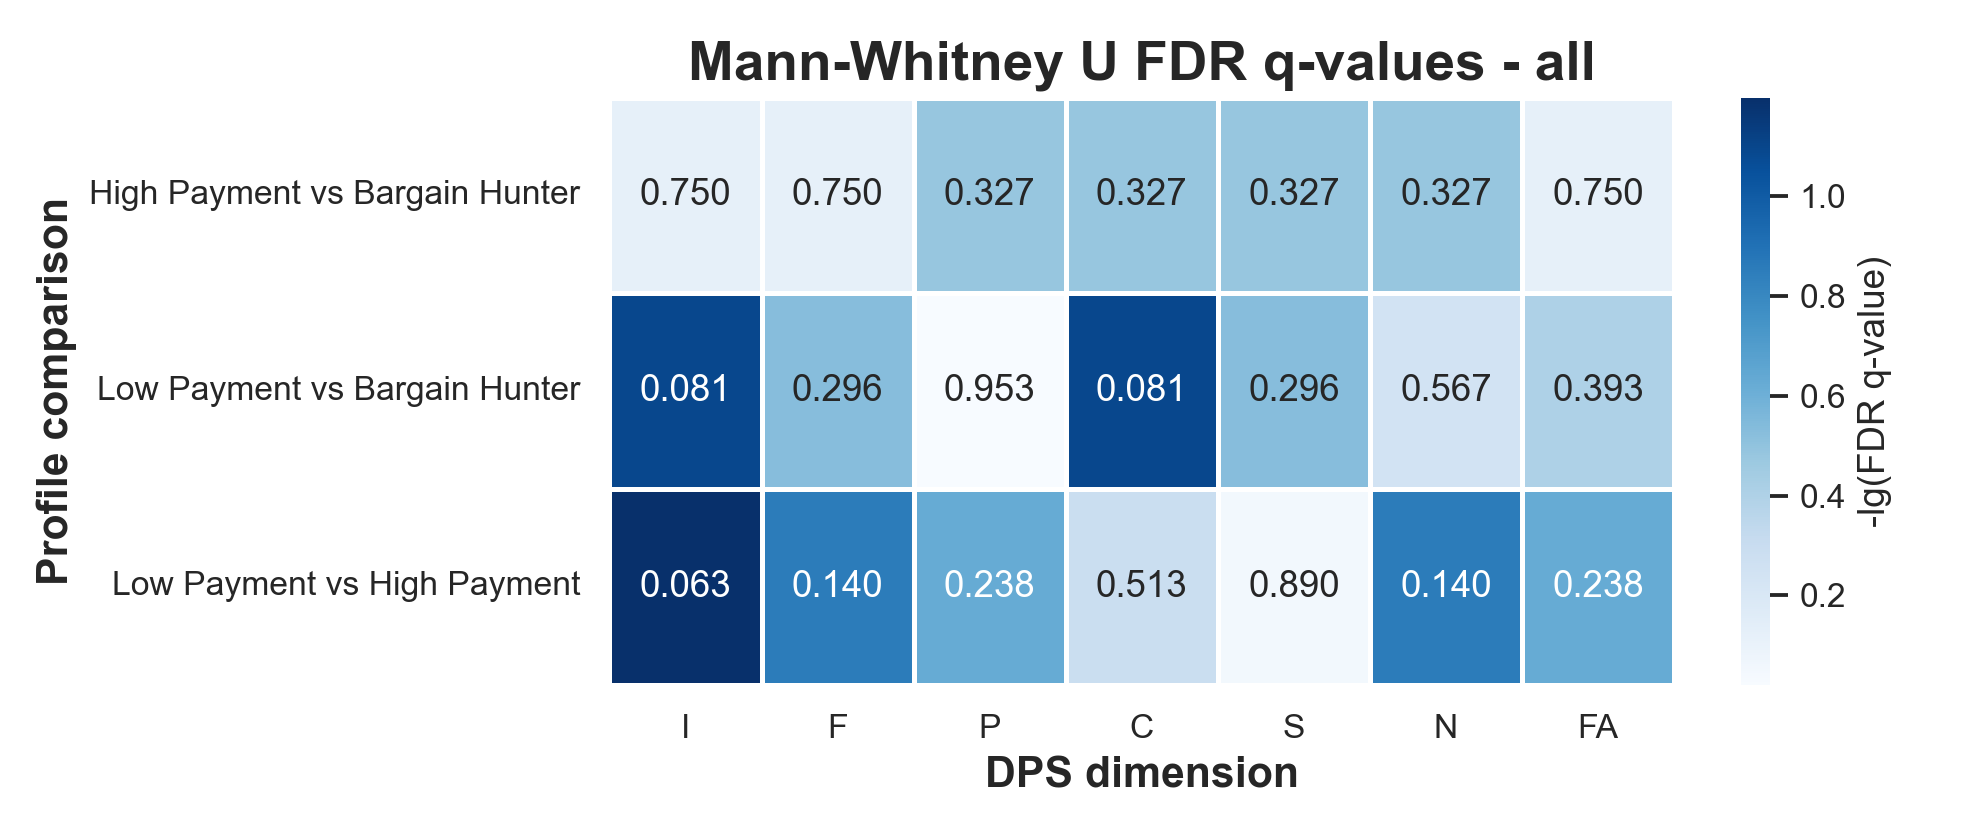
\includegraphics[width=0.95\linewidth]{figures/statistics/mannwhitney_qvalue_heatmap_all.png}
    \caption{Mann-Whitney U BH FDR q-value heatmap for raw DPS intensity comparisons across all audited applications.}
    \label{fig:qvalue-all-appendix}
\end{figure}

\begin{figure}[htbp]
    \centering
    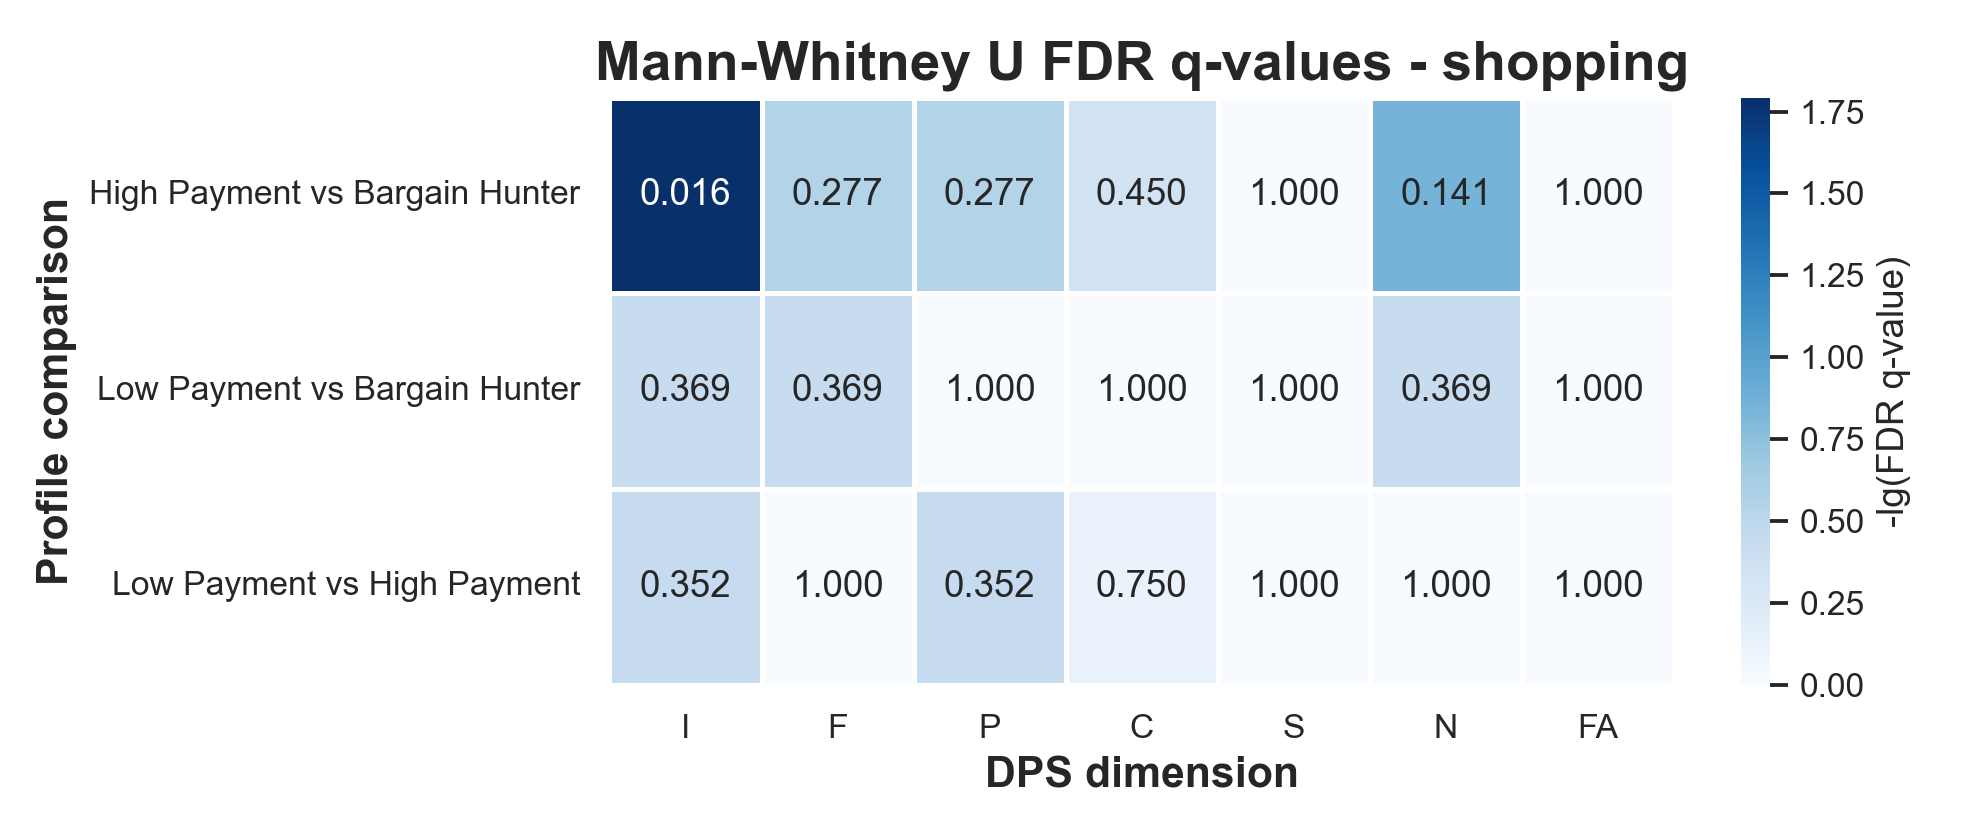
\includegraphics[width=0.95\linewidth]{figures/statistics/mannwhitney_qvalue_heatmap_shopping.png}
    \caption{Mann-Whitney U BH FDR q-value heatmap for raw DPS intensity comparisons in shopping applications.}
    \label{fig:qvalue-shopping}
\end{figure}

\begin{figure}[htbp]
    \centering
    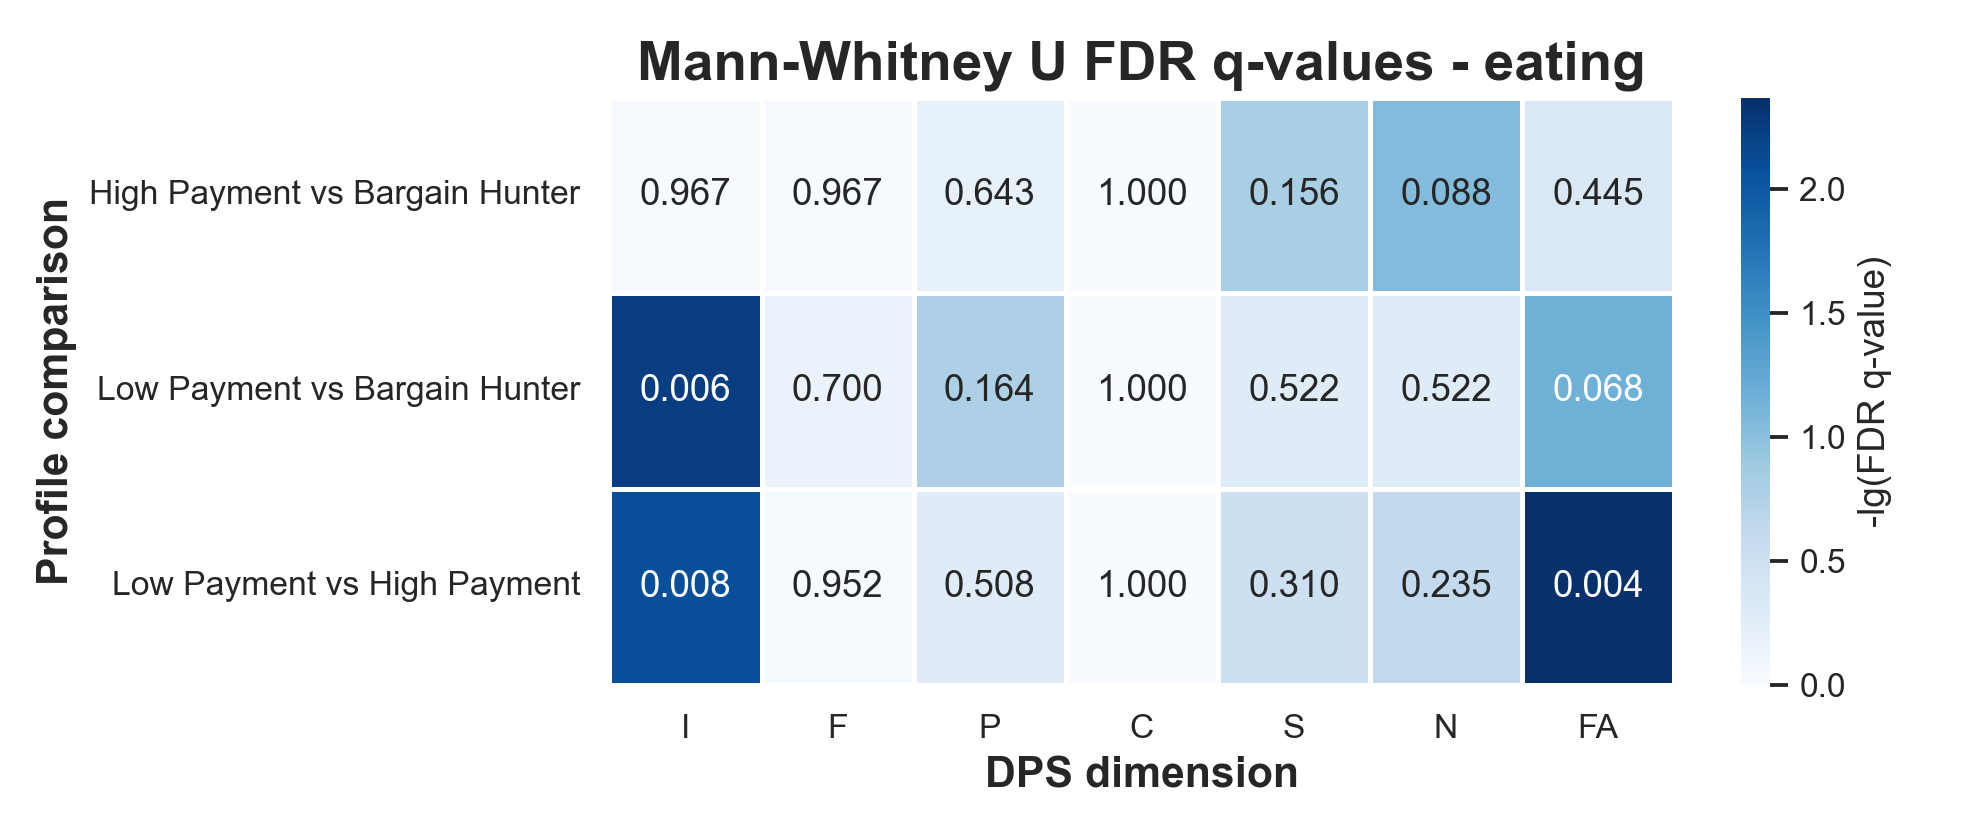
\includegraphics[width=0.95\linewidth]{figures/statistics/mannwhitney_qvalue_heatmap_eating.png}
    \caption{Mann-Whitney U BH FDR q-value heatmap for raw DPS intensity comparisons in food-delivery and eating-related applications.}
    \label{fig:qvalue-eating}
\end{figure}

\begin{figure}[htbp]
    \centering
    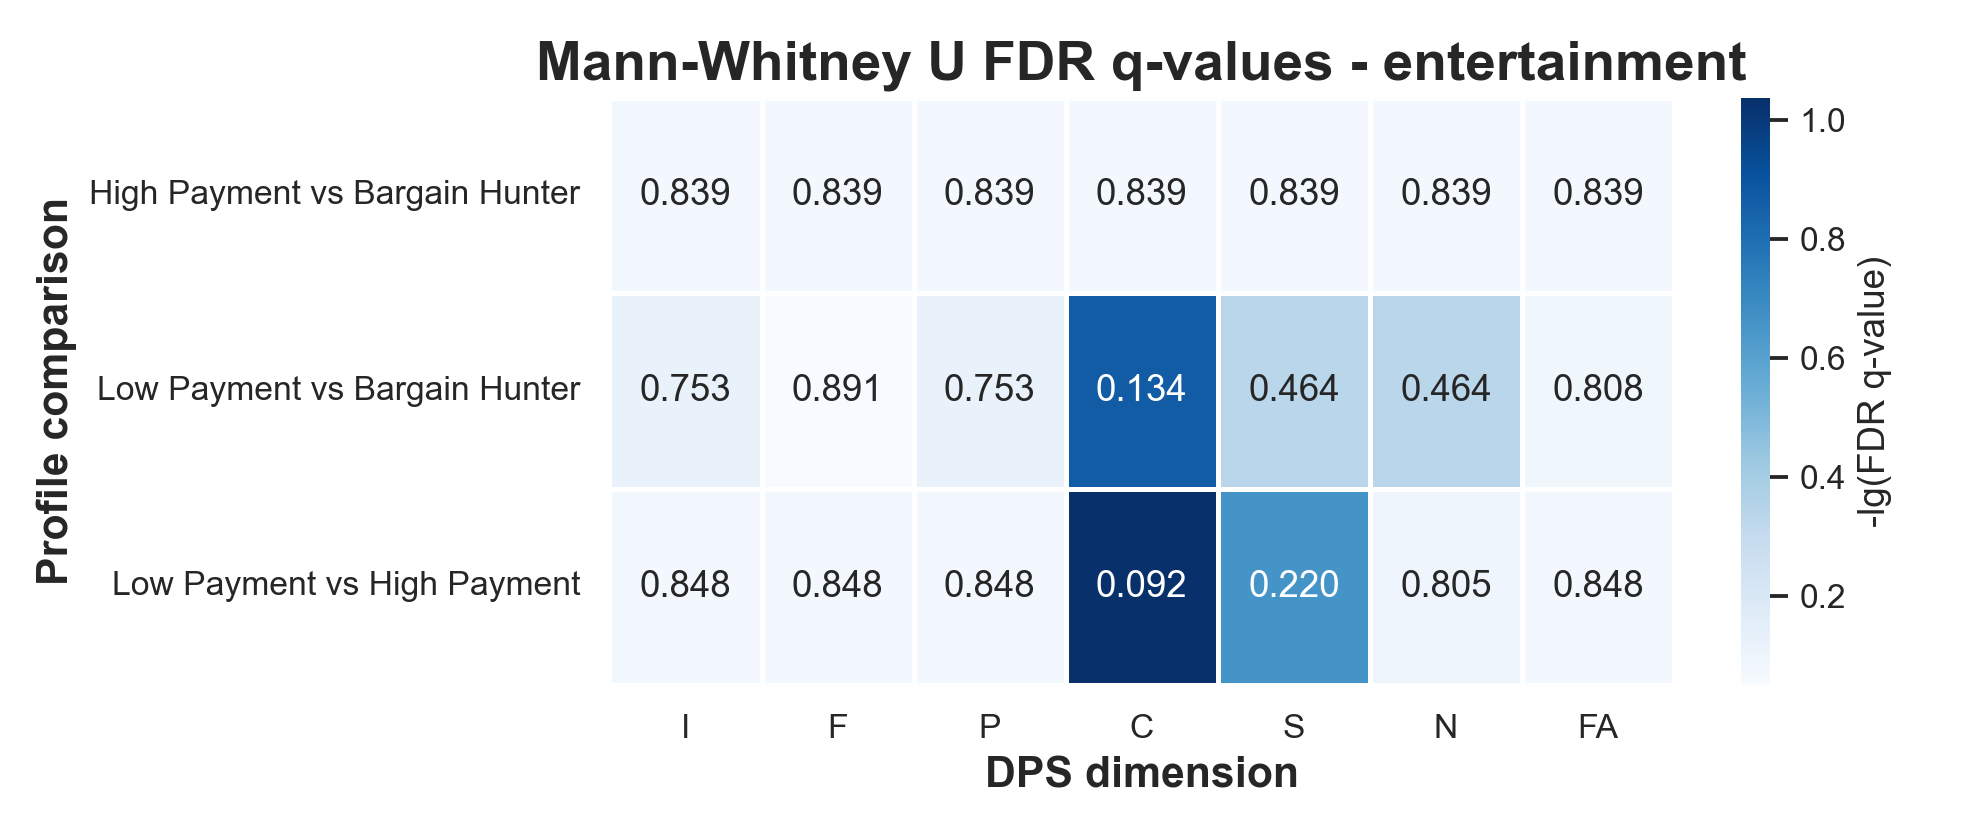
\includegraphics[width=0.95\linewidth]{figures/statistics/mannwhitney_qvalue_heatmap_entertainment.png}
    \caption{Mann-Whitney U BH FDR q-value heatmap for raw DPS intensity comparisons in entertainment applications.}
    \label{fig:qvalue-entertainment}
\end{figure}

\begin{figure}[htbp]
    \centering
    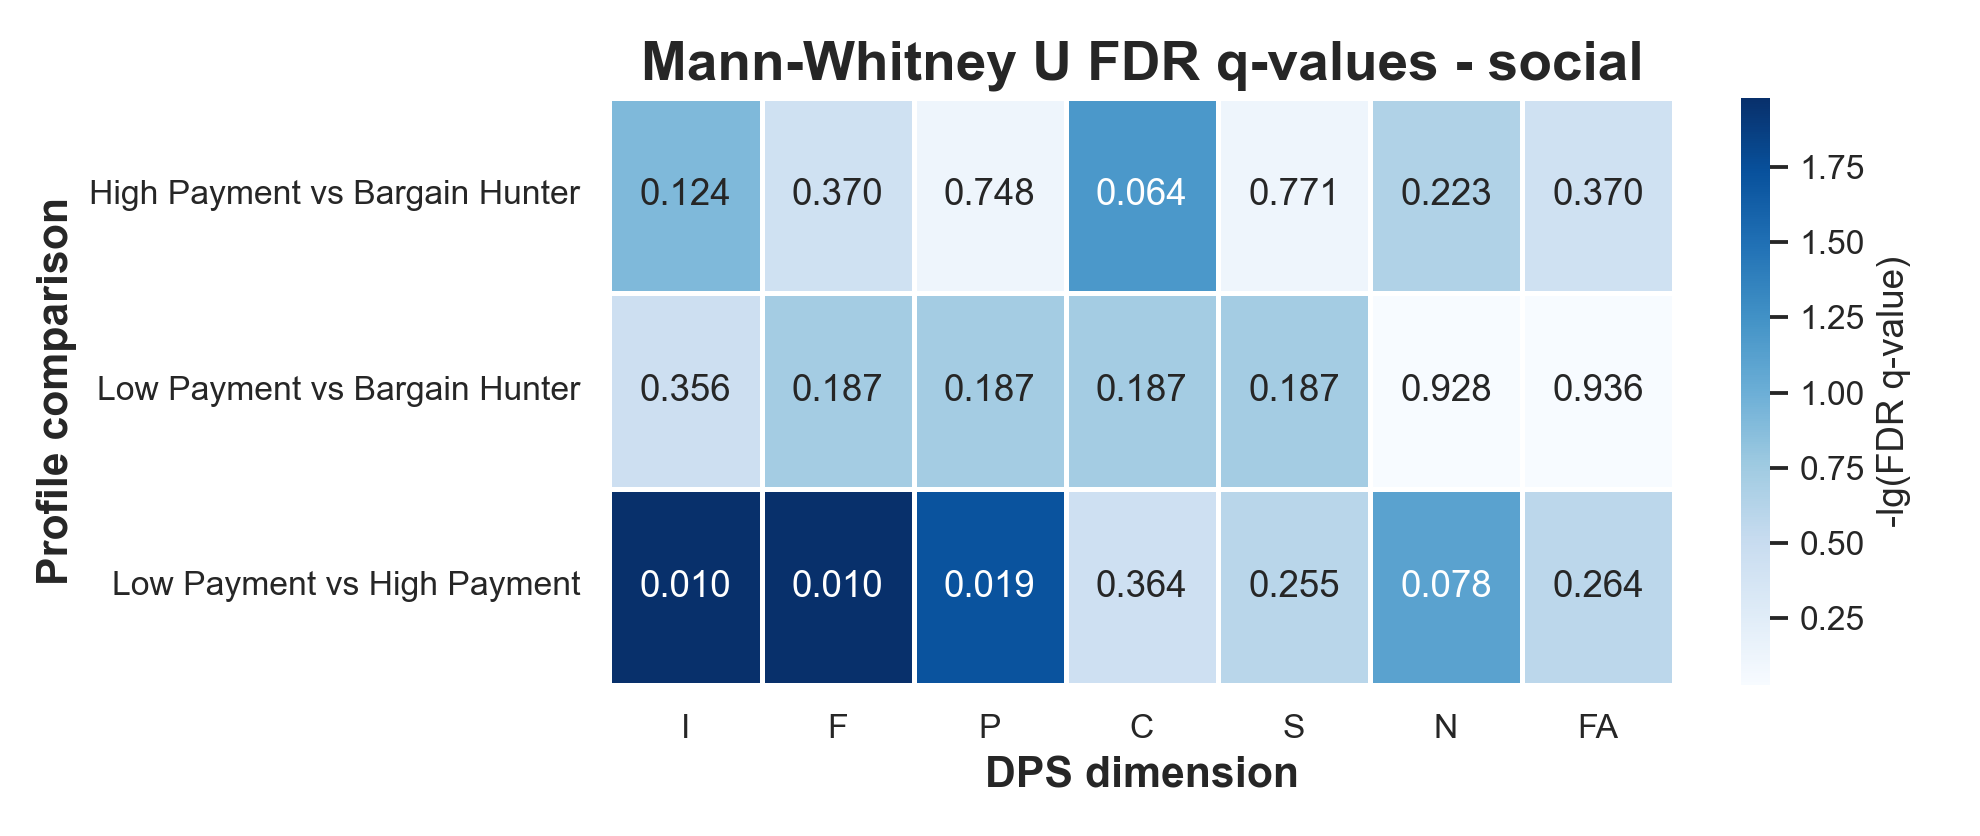
\includegraphics[width=0.95\linewidth]{figures/statistics/mannwhitney_qvalue_heatmap_social.png}
    \caption{Mann-Whitney U BH FDR q-value heatmap for raw DPS intensity comparisons in social applications.}
    \label{fig:qvalue-social}
\end{figure}

\begin{figure}[htbp]
    \centering
    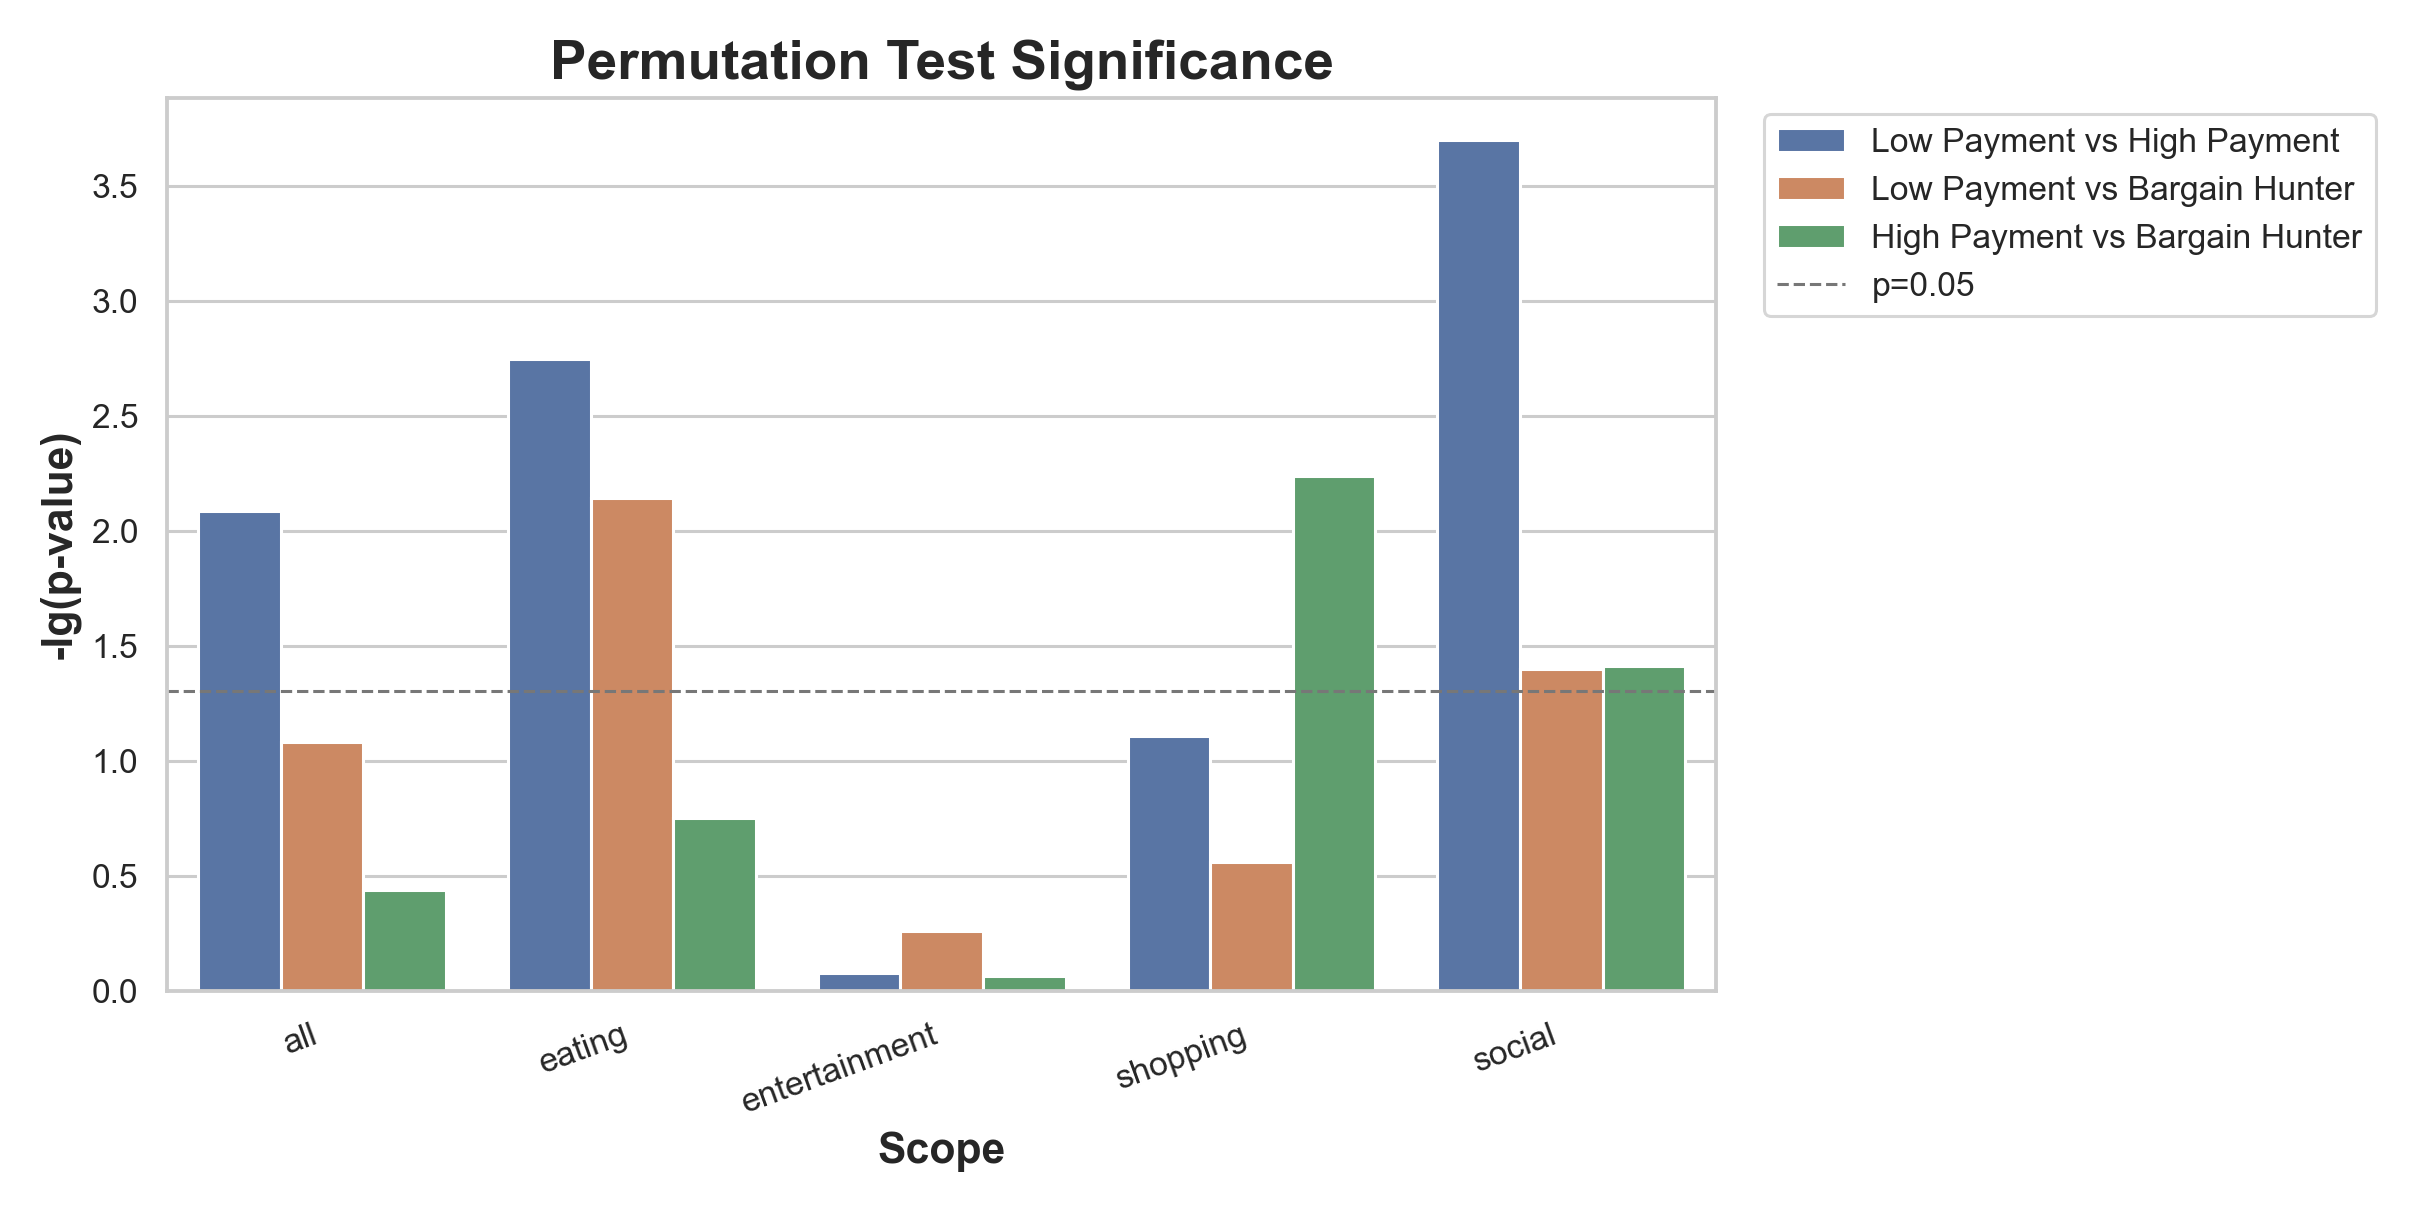
\includegraphics[width=0.95\linewidth]{figures/statistics/permutation_pvalues_by_scope.png}
    \caption{Permutation-test p-values by comparison scope based on binarized occurrence \(D_i>0\).}
    \label{fig:permutation-pvalues-appendix}
\end{figure}

\begin{figure}[htbp]
    \centering
    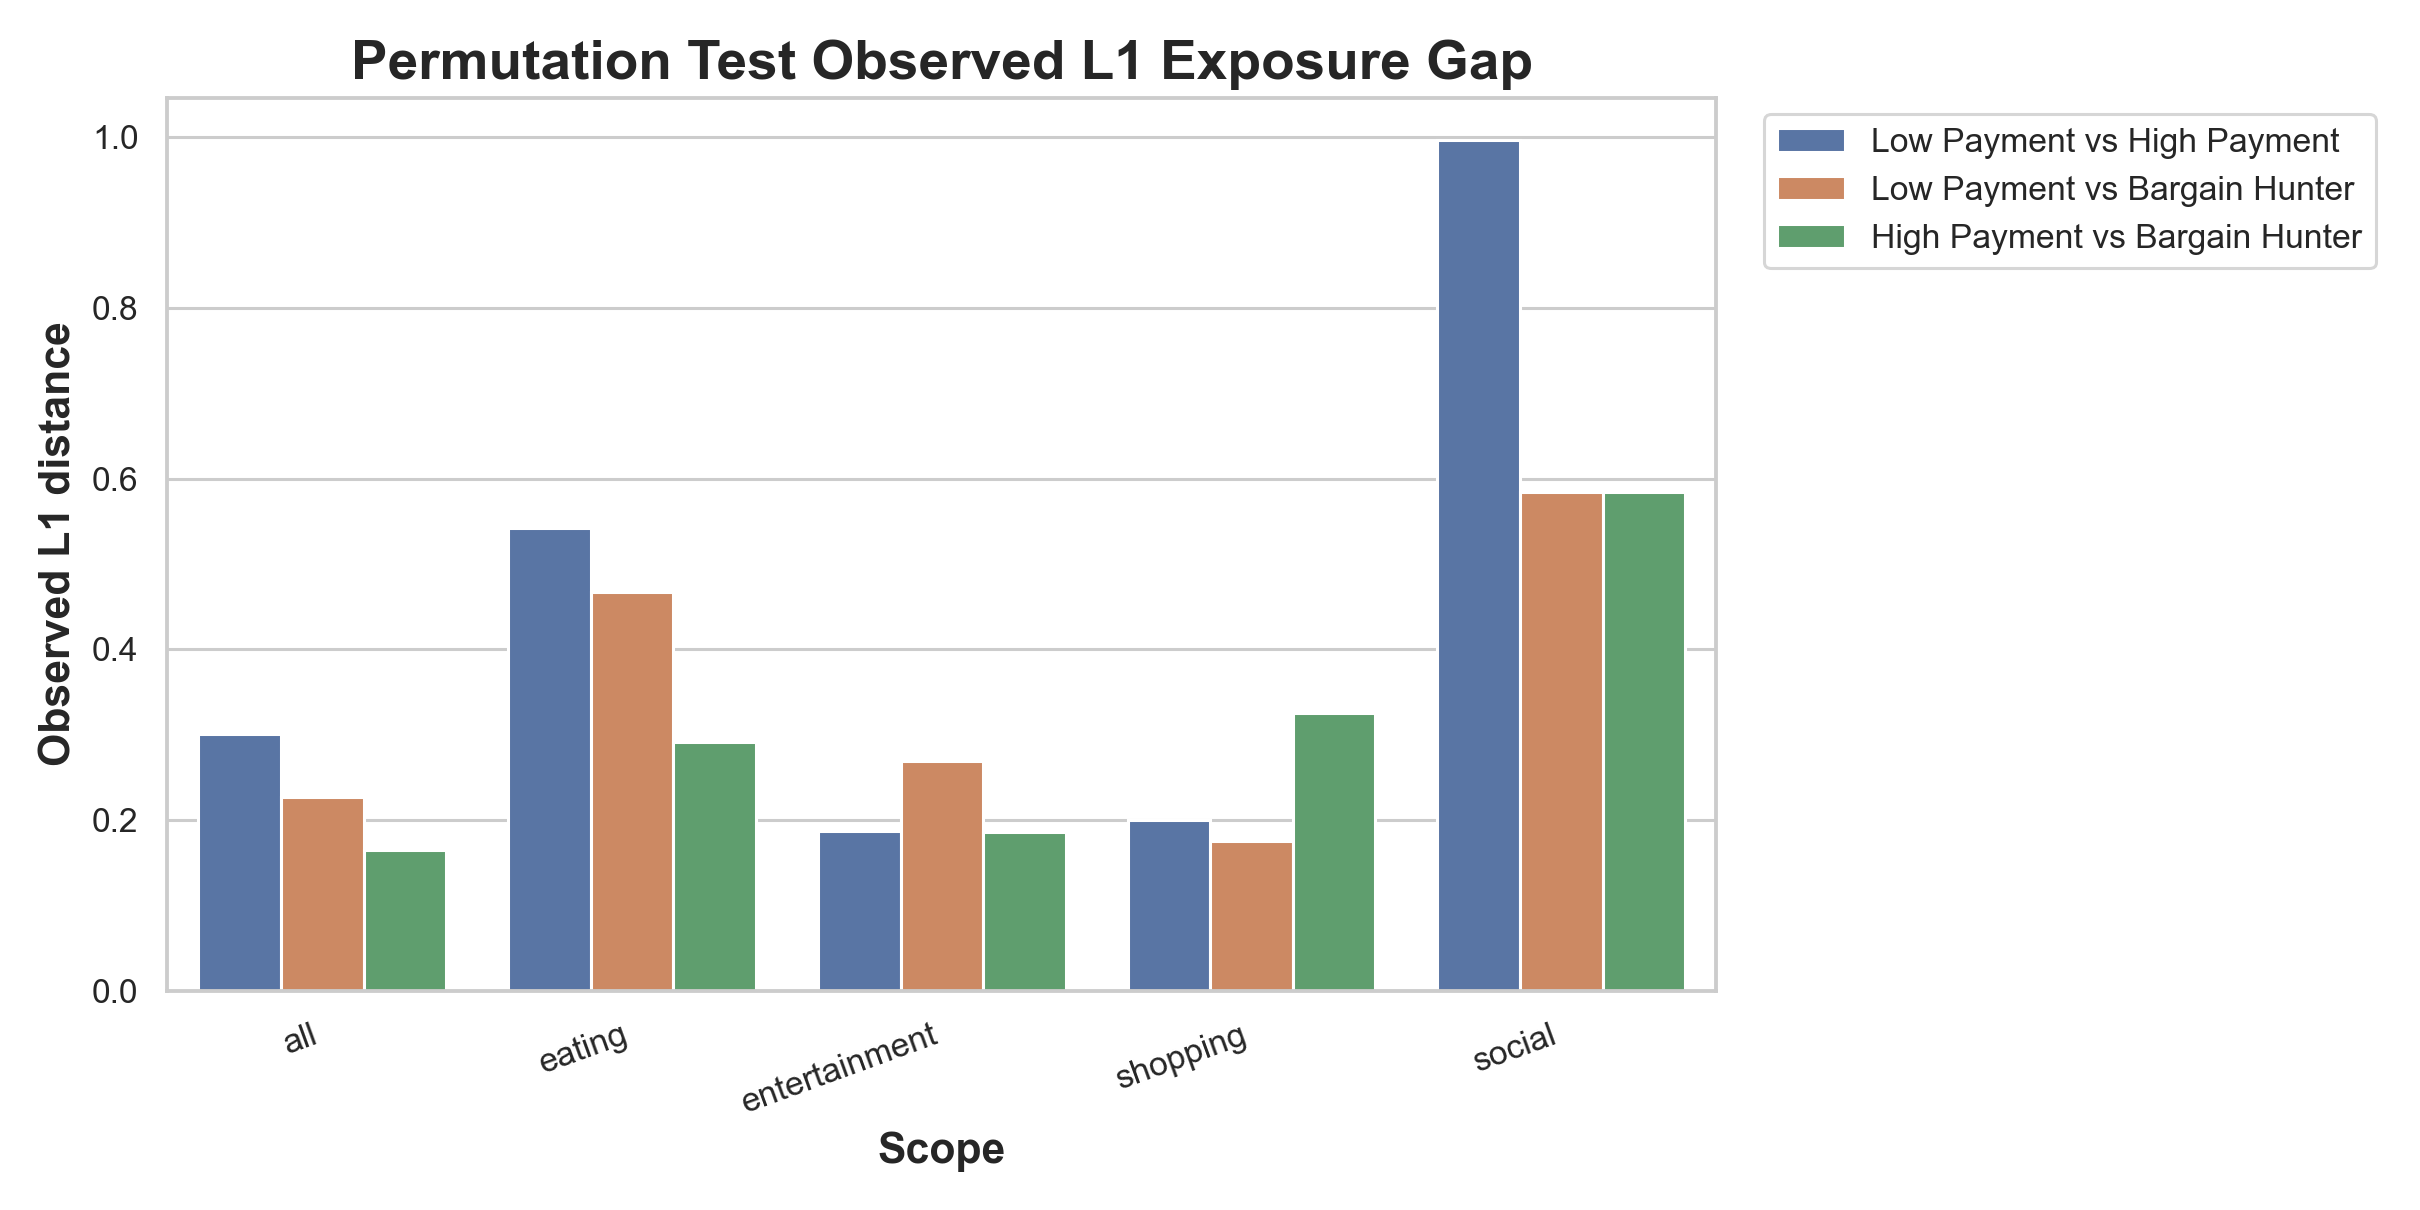
\includegraphics[width=0.95\linewidth]{figures/statistics/permutation_observed_l1_by_scope.png}
    \caption{Observed \(L_1\) exposure distances by comparison scope based on binarized occurrence \(D_i>0\).}
    \label{fig:permutation-l1-appendix}
\end{figure}

\begin{figure}[htbp]
    \centering
    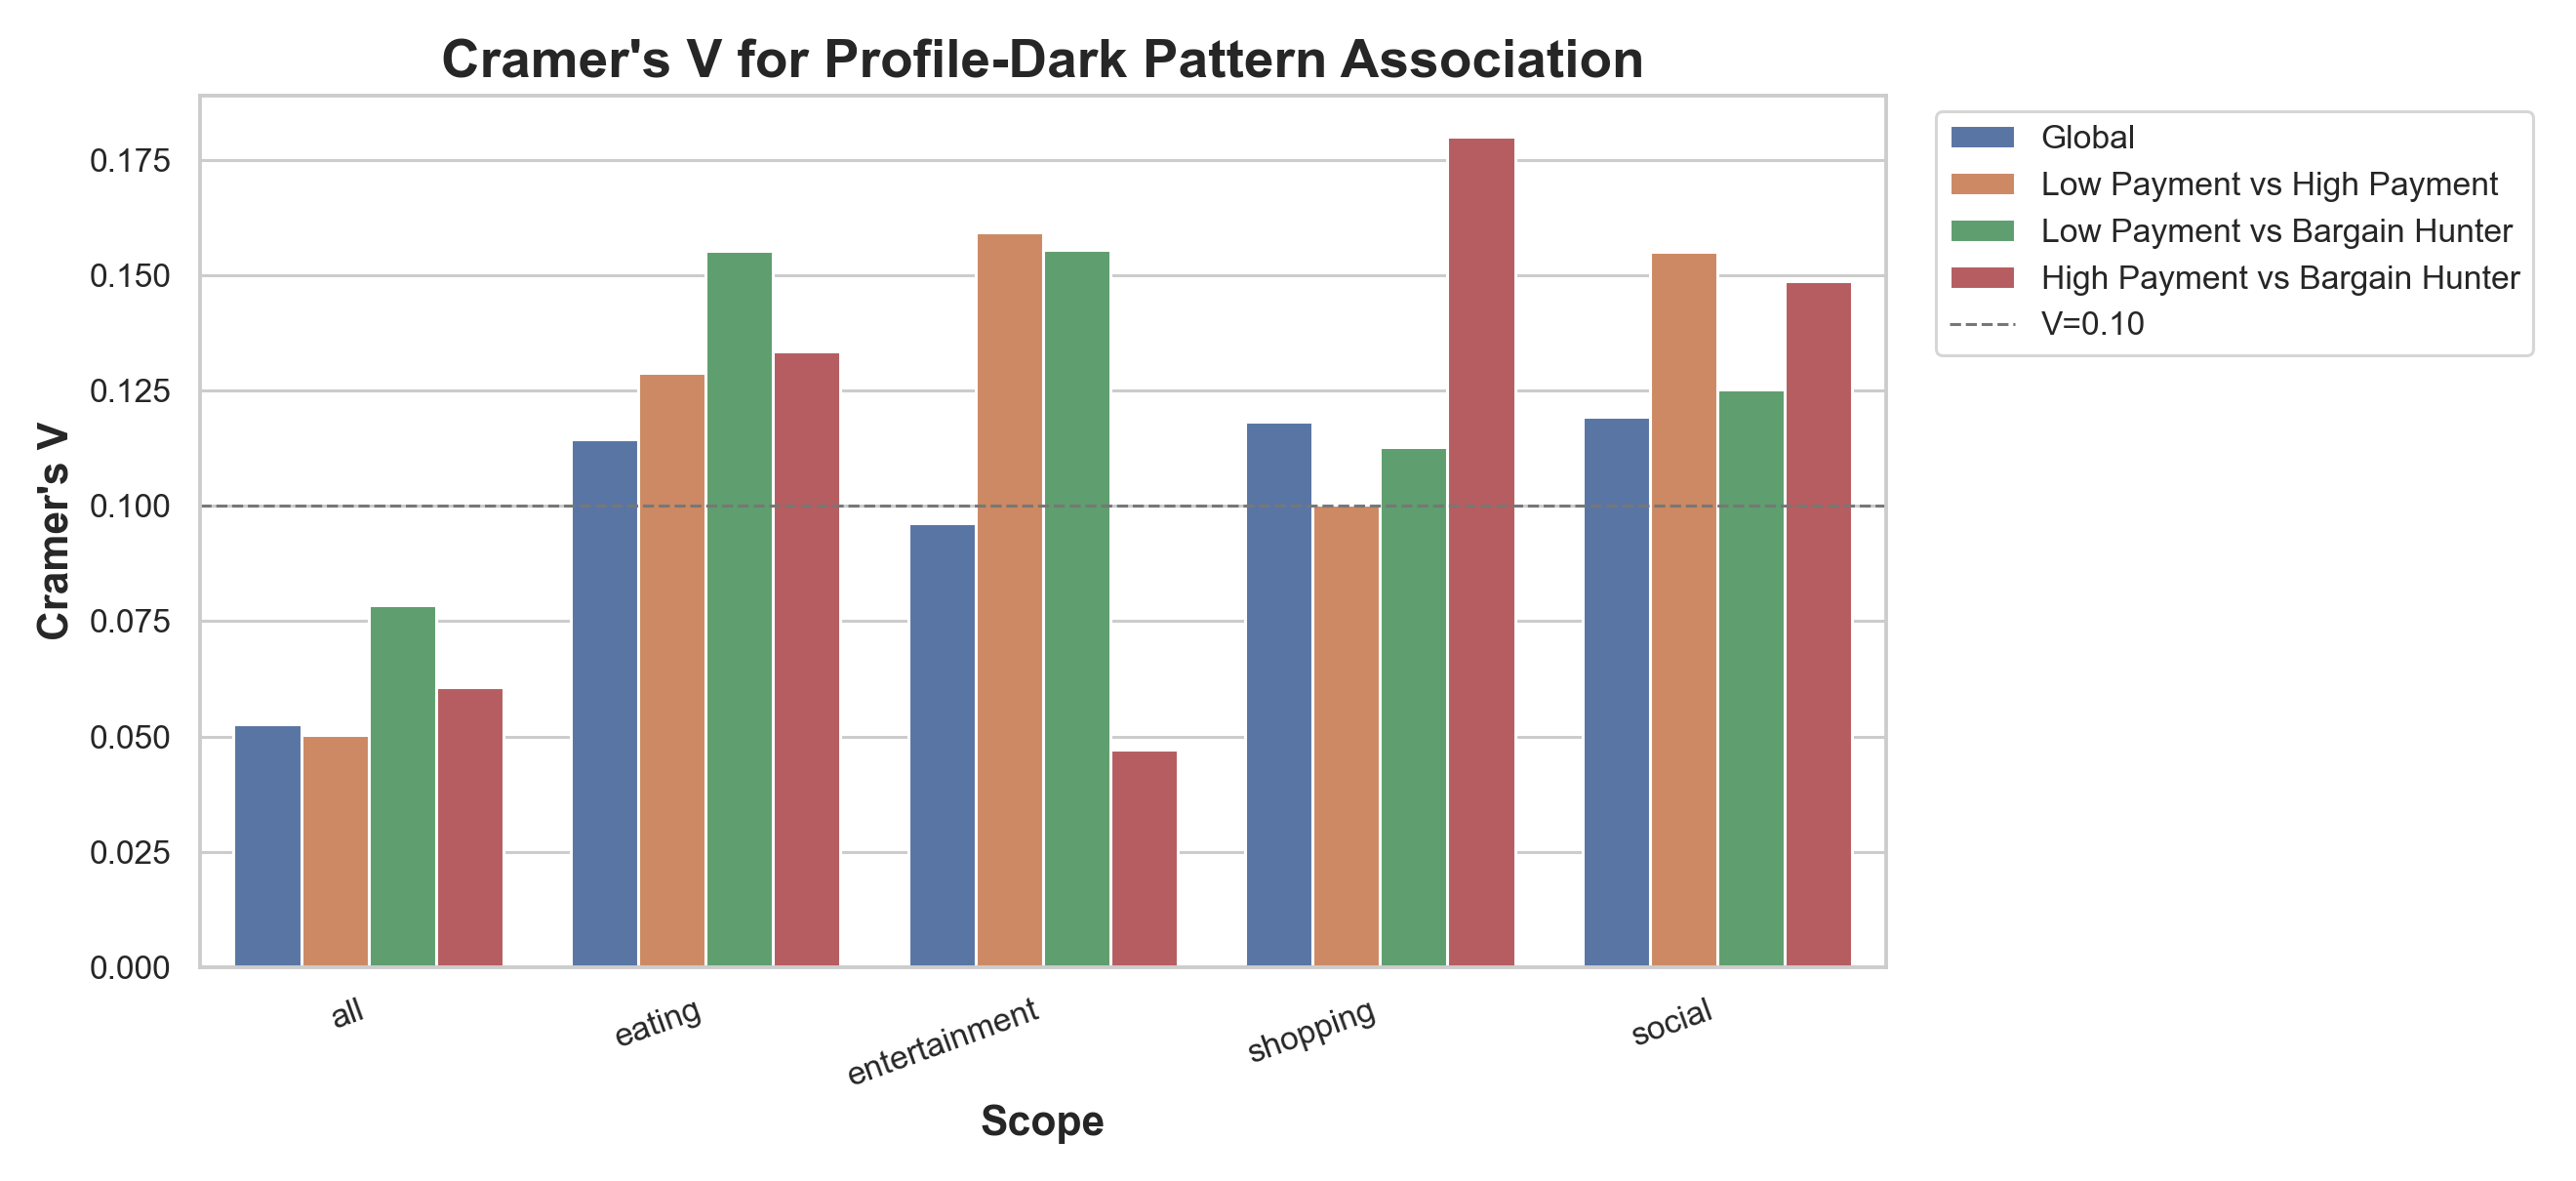
\includegraphics[width=0.95\linewidth]{figures/statistics/cramers_v_by_scope.png}
    \caption{Cramér's \(V\) association strength by comparison scope based on binarized occurrence \(D_i>0\).}
    \label{fig:cramers-v-appendix}
\end{figure}

The full convergence curves are interpreted as descriptive stability evidence rather than proof of causal convergence. If the running mean becomes less volatile after repeated interactions, this suggests that the target interaction budget is sufficient to produce a more stable estimate of profile-conditioned exposure within the archived trajectory. However, longer-term interaction histories may still reveal additional exposure dynamics.

\section{Appendix F: Statistical Validation Notes}
\label{app:statistical-validation-tables}

Appendix F documents how the statistical validation results are interpreted. The main report and Appendix~\ref{app:statistical-visualizations} report the exported plots for p-values, q-values, L1 distance, and Cramér's \(V\). These plots are read together rather than as independent proof from any single statistic.

The statistical validation is presented as evidence of association rather than causation. Since the experiment compares controlled profile-conditioned interaction traces, significant differences indicate that observed exposure patterns are unlikely to be explained solely by random profile assignment under the tested conditions. They are not interpreted as proving that the application intentionally targets a particular user group.

The permutation test summary describes how profile labels are randomly reassigned to construct a null distribution of exposure differences. The observed exposure gap is then compared against this null distribution. Low permutation p-values suggest that the observed gap is unusually large under random reassignment, while larger p-values suggest weaker evidence for a profile-associated difference.

In addition to statistical significance, the appendix reports practical difference measures. The \(L_1\) distance between two profile-level DPS exposure vectors is used to describe the magnitude of exposure difference:
\[
L_1(A_i, A_j) = \sum_{d \in DPS} 
\left| E(D_d \mid A_i) - E(D_d \mid A_j) \right|.
\]
Cramér's \(V\) can be used to summarize the strength of association between profile type and DPS exposure for categorical or discretized annotations. In this report, the contingency table is built from binarized DPS presence, so each dimension is first reduced to present versus absent before the counts are aggregated by profile. If future work adopts an ordinal 0/1/2 scheme, the positive levels should be collapsed into the presence category for this statistic or analyzed with a separate ordinal association measure. Reporting both significance and effect-size-oriented metrics helps avoid overinterpreting small but statistically detectable differences.

Together, these validation outputs provide empirical support for the report's main claim that dark pattern exposure can be estimated as a profile-conditioned outcome. The results should be discussed as observed differences under controlled audit conditions, rather than as direct evidence of intent or demographic discrimination.
